\newtheorem*{remark}{Remark}
% % \newcommand{\dotprod}[2]{#1 \cdot #2}
\newcommand{\dotprod}{ \cdot }

\newcommand{\colvec}[1]{\ensuremath{\begin{pmatrix}#1\end{pmatrix}}}


% \newcount\colveccount

% \newcommand*\colvec[1]{
        % \global\colveccount#1
        % \begin{pmatrix}
        % \colvecnext
% }

%%%%%%%%%%%%%%%%%%%%%%%%%%%%%%%%%%%%%%%%%%%%%%%%%%%%%%%%%%%%%%%%%%%%%%%%%%%%%%%%%%
\begin{frame}[fragile]\frametitle{}
\begin{center}
{\Large Vector Spaces }
\end{center}
\end{frame}



%%%%%%%%%%%%%%%%%%%%%%%%%%%%%%%%%%%%%%%%%%%%%%%%%%%%%%%%%%%%%%%%%%%%%%%%%%%%%%%%%%
\begin{frame}[fragile]
\frametitle{Background}
\begin{itemize}
\item Vectors are generally represented by list of numbers, these are coefficients of the basis vectors. For 2D, x and y axes are basis and coefficients are the coordinates.
\item We can have n-dimensional vector representing point in n-dimensional space.
\item Determinant (area notion) and eigen vectors (principal direction) are independent of the basis vectors ie the coordinate system, ie. they have some spatial ie space-ness properties.
\item SImilarly even ``functions'' behave similarly. Instead of discrete numbers like earlier, they represent continuous numbers. But the space-ness remains.
\item The way you can add two vectors, you can add two functions. As you can scale a vector, you can scale a function. The resultant function curves just add up or scale respectively.
\end{itemize}


\tiny{(Ref: Abstract vector spaces | Chapter 16, Essence of linear algebra - 3Blue1Brown)}


\end{frame}

%%%%%%%%%%%%%%%%%%%%%%%%%%%%%%%%%%%%%%%%%%%%%%%%%%%%%%%%%%%%%%%%%%%%%%%%%%%%%%%%%%
\begin{frame}[fragile]
\frametitle{Background}
\begin{itemize}
\item Addition and scaling thus is common to vectors and function.
\item Linear combination has both addition and scaling. Its a Transformation or Operator.
\item Transformation is linear if it satisfies two properties : addition and scaling.
\item Scaling of an addition is addition of the scaled vectors.
\item Transformation of vectors can also be done by representing it in a transformed coordinate system (ie basis vectors)
\item This is true for vectors as well as functions.
\item Derivatives also has additive and scaling properties. Meaning, derivative of an addition is addition of the derivatives. Same for scaling.
\end{itemize}

\tiny{(Ref: Abstract vector spaces | Chapter 16, Essence of linear algebra - 3Blue1Brown)}

\end{frame}

%%%%%%%%%%%%%%%%%%%%%%%%%%%%%%%%%%%%%%%%%%%%%%%%%%%%%%%%%%%%%%%%%%%%%%%%%%%%%%%%%%
\begin{frame}[fragile]
\frametitle{Background}

Derivative is Linear

\begin{center}
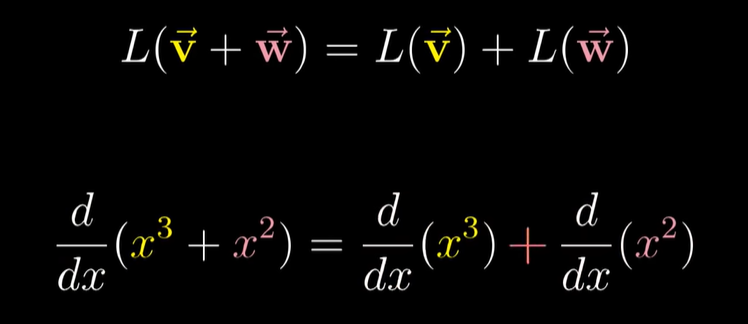
\includegraphics[width=0.5\linewidth,keepaspectratio]{vecspaces1}

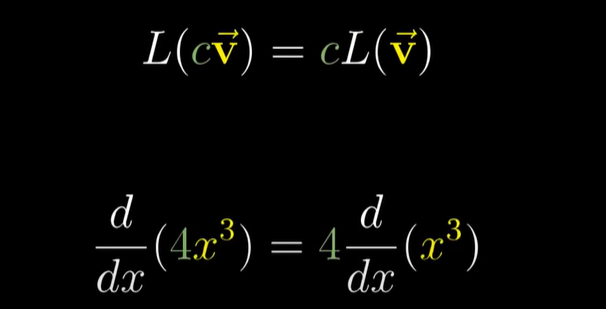
\includegraphics[width=0.5\linewidth,keepaspectratio]{vecspaces2}
\end{center}


\tiny{(Ref: Abstract vector spaces | Chapter 16, Essence of linear algebra - 3Blue1Brown)}

\end{frame}

%%%%%%%%%%%%%%%%%%%%%%%%%%%%%%%%%%%%%%%%%%%%%%%%%%%%%%%%%%%%%%%%%%%%%%%%%%%%%%%%%%
\begin{frame}[fragile]
\frametitle{Background}

Polynomials can also be represented as coefficients of basis having powers of $x$.

\begin{center}
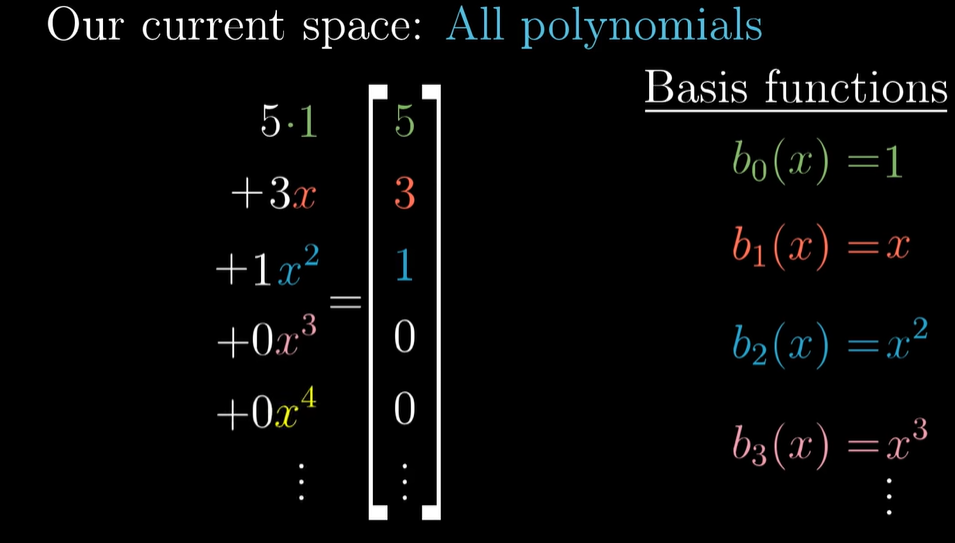
\includegraphics[width=0.5\linewidth,keepaspectratio]{vecspaces3}
\end{center}

Vectors and functions have similar options.

\begin{center}
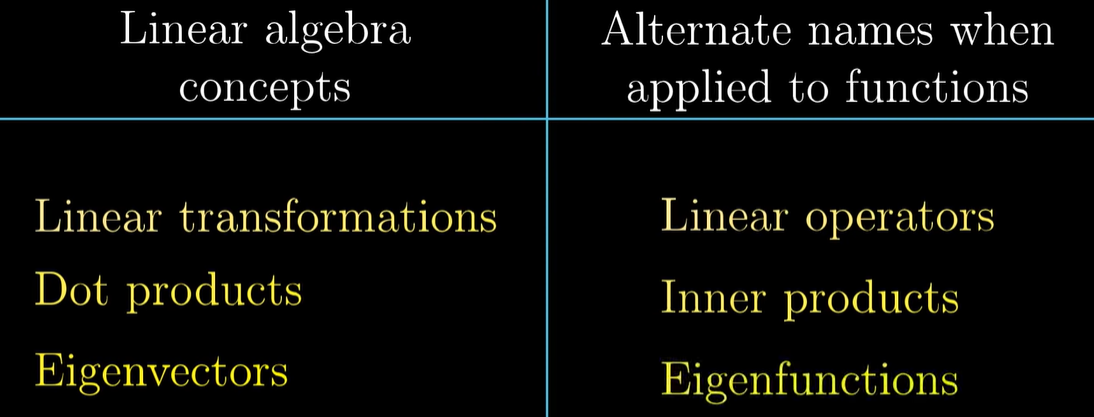
\includegraphics[width=0.5\linewidth,keepaspectratio]{vecspaces4}
\end{center}

\tiny{(Ref: Abstract vector spaces | Chapter 16, Essence of linear algebra - 3Blue1Brown)}

\end{frame}

%%%%%%%%%%%%%%%%%%%%%%%%%%%%%%%%%%%%%%%%%%%%%%%%%%%%%%%%%%%%%%%%%%%%%%%%%%%%%%%%%%
\begin{frame}[fragile]
\frametitle{Background}

\begin{itemize}
\item So many things are Vector-ish, adhering to Learning Transformation.
\item Thus all those have been abstracted as a structure called ``Vector Spaces''. Thus while developing further theory, we do not have to think about actual reincarnations.
\item So a set of rules (called `Axioms') are decided to define the ``Vector Spaces''.
\item Axioms are interfaces or protocols, whoever abides by them can thus be applicable in the further theory or proofs.
\end{itemize}

\begin{center}
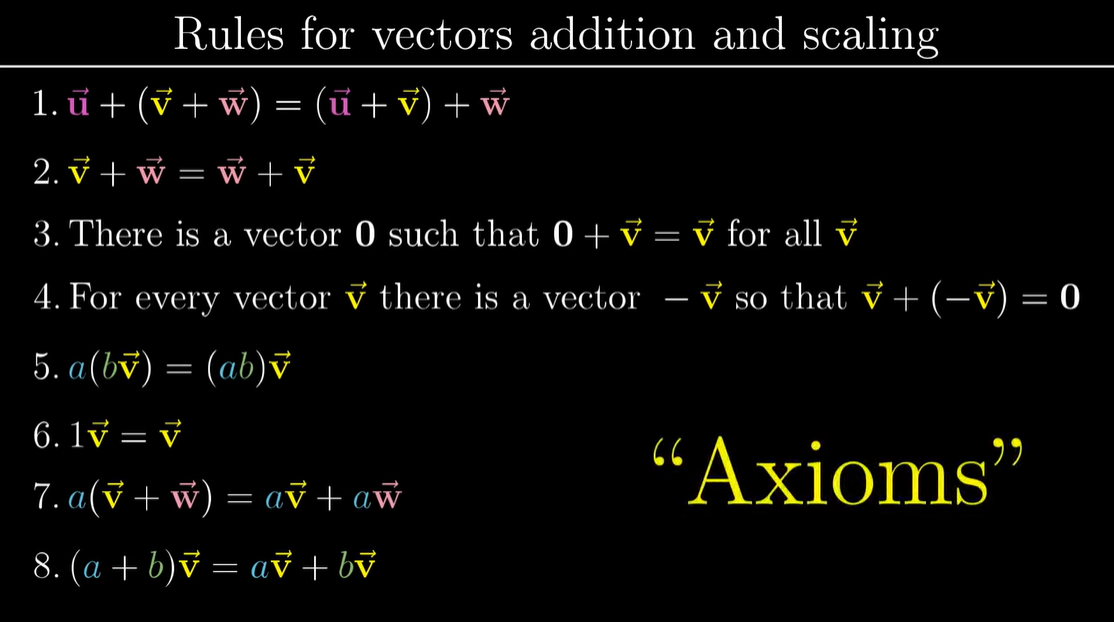
\includegraphics[width=0.5\linewidth,keepaspectratio]{vecspaces5}
\end{center}

\tiny{(Ref: Abstract vector spaces | Chapter 16, Essence of linear algebra - 3Blue1Brown)}

\end{frame}

%%%%%%%%%%%%%%%%%%%%%%%%%%%%%%%%%%%%%%%%%%%%%%%%%%%%%%%%%%%%%%%%%%%%%%%%%%%%%%%%%%
\begin{frame}[fragile]
\frametitle{Background}

\begin{center}
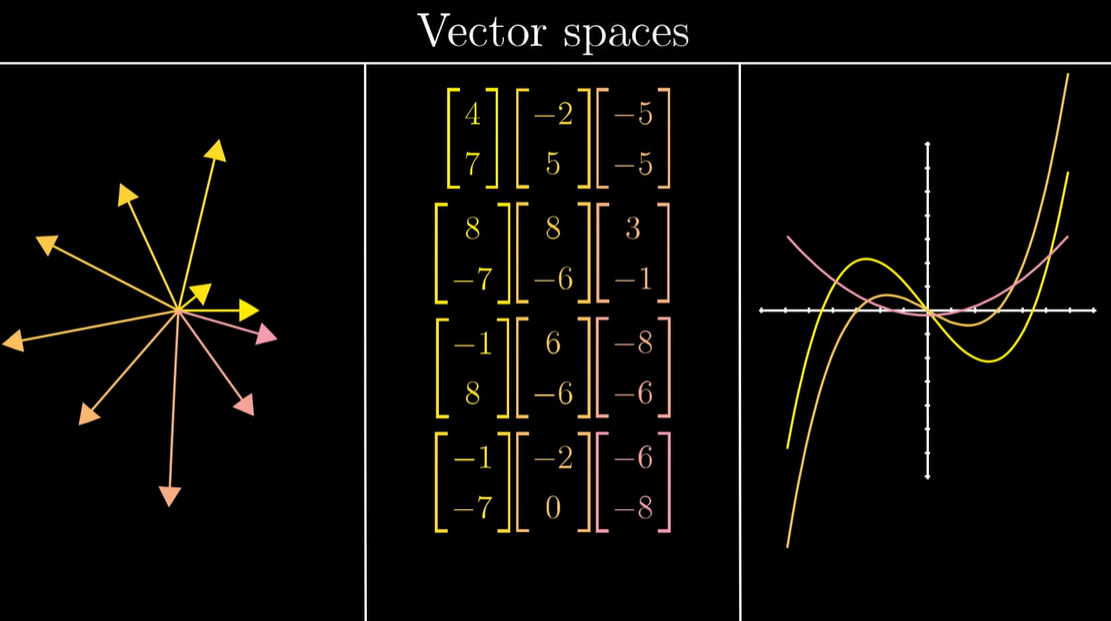
\includegraphics[width=\linewidth,keepaspectratio]{vecspaces6}
\end{center}

\tiny{(Ref: Abstract vector spaces | Chapter 16, Essence of linear algebra - 3Blue1Brown)}

\end{frame}




%%%%%%%%%%%%%%%%%%%%%%%%%%%%%%%%%%%%%%%%%%%%%%%%%%%%%%%%%%%%%%%%%%%%%%%%%%%%%%%%%%
\begin{frame}[fragile]
\frametitle{What determines a vector space?}

\begin{itemize}
\item A nonempty set $V$ whose elements are called {\em vectors}.
\item An operation $+$ called vectors addition, such that $$ \text{ vector } + \text{ vector } = \text{ vector }$$ 
In other words, we have {\em closure} under vector addition.
\item An operation $\cdot$ called scalar multiplication, such that $$ \text{ scalar } \cdot \text{ vector } = \text{ vector }$$ 
In other words, we have {\em closure} under scalar multiplication.
\item The remaining 8 axioms are all satisfied. 
\end{itemize}
\end{frame}

%%%%%%%%%%%%%%%%%%%%%%%%%%%%%%%%%%%%%%%%%%%%%%%%%%%%%%%%%%%%%%%%%%%%%%%%%%%%%%%%%%
\begin{frame}[fragile]
\frametitle{Some basic identities in a vector space}

\textbf{Theorem}: Let $V$ be a vector space. The following statements are always true.

\begin{itemize}
\item[a)] $\displaystyle 0 \cdot \vec{u} = \vec{0}$

\item[b)] $\displaystyle k \cdot \vec{0} = \vec{0}$

\item[c)] $\displaystyle (-1) \cdot \vec{u} = - \vec{u}$

\item[d)] If $\displaystyle k \cdot \vec{u} = \vec{0}$ then $k=0$ or $\vec{u} = \vec{0}$.

\end{itemize}

\end{frame}


%%%%%%%%%%%%%%%%%%%%%%%%%%%%%%%%%%%%%%%%%%%%%%%%%%%%%%%%%%%%%%%%%%%%%%%%%%%%%%%%%%
\begin{frame}[fragile]
\frametitle{Vector subspace}

Let $(V, +, \cdot)$ be a vector space.



\textbf{Definition}:  A subset $W$ of $V$ is called a {\em subspace} if $W$ is itself a vector space with the operations $+$ and $\cdot$ defined on $V$.



\textbf{Theorem}: Let $W$ be a nonempty subset of $V$. Then $W$ is a subspace of $V$ if and only if it is {\em closed} under addition and scalar multiplication, in other words, if:

\begin{itemize}
\item[i.)] For any $\vec{u}, \vec{v}$ in $W$, we have $\vec{u} + \vec{v}$ is in $W$.

\item[ii.)] For any scalar $k$ and any vector $\vec{u}$ in $W$ we have $k \cdot \vec{u}$ is in $W$.
\end{itemize}
 

\end{frame}


%%%%%%%%%%%%%%%%%%%%%%%%%%%%%%%%%%%%%%%%%%%%%%%%%%%%%%%%%%%%%%%%%%%%%%%%%%%%%%%%%%
\begin{frame}[fragile]
\frametitle{Linear combinations and the span of a set of vectors}

Let $(V, +, \cdot)$ be a vector space.



\textbf{Definition}: Let $\vec{v}$ be a vector in $V$. We say that $\vec{v}$ is a {\em linear combination} of the vectors $\vec{v_1}, \vec{v_2}, \ldots, \vec{v_r}$ if there are scalars $k_1, k_2, \ldots, k_r$ such that
$$\vec{v} = k_1 \cdot \vec{v_1} + k_2 \cdot \vec{v_2} + \ldots + k_r \cdot \vec{v_r}$$

The scalars $k_1, k_2, \ldots, k_r$ are called the {\em coefficients} of the linear combination.





\textbf{Definition}: Let $S = \{ \vec{v_1}, \vec{v_2}, \ldots, \vec{v_r} \}$ be a set of vectors in $V$.

Let $W$ be the set of \textbf{all linear combinations} of $\vec{v_1}, \vec{v_2}, \ldots, \vec{v_r}$:
$$W = \{  k_1 \cdot \vec{v_1} + k_2 \cdot \vec{v_2} + \ldots + k_r \cdot \vec{v_r} \ \  \colon  \text{ for all choices of scalars } k_1, k_2, \ldots, k_r \}$$

Then $W$ is called the {\em span} of the set $S$.

We write:
$$W = \text{ span } S  \quad \text{ or } \quad W = \text{ span }   \{ \vec{v_1}, \vec{v_2}, \ldots, \vec{v_r} \}$$

\end{frame}


%%%%%%%%%%%%%%%%%%%%%%%%%%%%%%%%%%%%%%%%%%%%%%%%%%%%%%%%%%%%%%%%%%%%%%%%%%%%%%%%%%
\begin{frame}[fragile]
\frametitle{Linear combinations and the span of a set of vectors}

Let $(V, +, \cdot)$ be a vector space and let $S = \{ \vec{v_1}, \vec{v_2}, \ldots, \vec{v_r} \}$ be a set of vectors in $V$.

$$\text{span} S = \{  k_1 \cdot \vec{v_1} + k_2 \cdot \vec{v_2} + \ldots + k_r \cdot \vec{v_r}  \ \colon  \text{ for all scalars } k_1, k_2, \ldots, k_r \}$$

(all linear combinations of $\vec{v_1}, \vec{v_2}, \ldots, \vec{v_r}$).

\bigskip


\textbf{Theorem}: $\text{ span }   \{ \vec{v_1}, \vec{v_2}, \ldots, \vec{v_r} \}$ is a subspace of $V$.

It is in fact the {\em smallest} subspace of $V$ that contains all vectors $\{ \vec{v_1}, \vec{v_2}, \ldots, \vec{v_r} \}$.

\end{frame}


%%%%%%%%%%%%%%%%%%%%%%%%%%%%%%%%%%%%%%%%%%%%%%%%%%%%%%%%%%%%%%%%%%%%%%%%%%%%%%%%%%
\begin{frame}[fragile]
\frametitle{Linear independence in a vector space $V$}

Let $V$ be a vector space and let $S = \{ \vec{v_1}, \vec{v_2}, \ldots, \vec{v_r} \}$ be a set of vectors in $V$.



\textbf{Definition}: The set  $S$ is called {\em linearly independent} if the vector equation
\begin{equation*}
(*) \quad  c_1 \cdot \vec{v_1} + c_2 \cdot \vec{v_2} + \ldots + c_r \cdot \vec{v_r} = \vec{0}
\end{equation*}


has \textbf{only one} solution, the trivial one:
$$c_1 = 0, \ c_2 = 0, \ \ldots, c_r = 0$$

The set is called linearly dependent otherwise, if equation (*) has other solutions besides the trivial one.

\textbf{Theorem}: The set of vectors $S$ is linearly independent if and only if \textbf{no} vector in the set is a linear combination of the other vectors in the set.

The set of vectors $S$ is linearly dependent if and only if one of the vectors in the set is a linear combination of the other vectors in the set.
\end{frame}




%%%%%%%%%%%%%%%%%%%%%%%%%%%%%%%%%%%%%%%%%%%%%%%%%%%%%%%%%%%%%%%%%%%%%%%%%%%%%%%%%%
\begin{frame}[fragile]
\frametitle{Introduction}
\begin{itemize}
\item Thus far we have thought of vectors as lists of numbers in $\mathbb{R}^n$.  
\item As it turns out, the idea of a vector can be much more general.  
\item In the spirit of generalization, then, we will define vectors based on their most important properties.  
\item Once complete, our new definition of vectors will include vectors in $\mathbb{R}^n$, but will also cover many other extremely useful notions of vectors. 
\item We do this in the hope of creating a mathematical structure
applicable to a wide range of real world problems.
\item The two key properties of vectors are that they can be added together and multiplied by scalars.  
\end{itemize}

Over to definition \ldots

\tiny{(Ref: Linear Algebra - UCDavis, David Cherney, Tom Denton, Rohit Thomas and Andrew Waldron)}


\end{frame}

%%%%%%%%%%%%%%%%%%%%%%%%%%%%%%%%%%%%%%%%%%%%%%%%%%%%%%%%%%%%%%%%%%%%%%%%%%%%%%%%%%
\begin{frame}[fragile]
\frametitle{Definition}

\begin{definition} A \emph{vector space}\index{Vector space} (over $\mathbb{R}$) is a set $V$ with two operations $+$ and $\cdot$ satisfying the following properties for all $u, v \in V$ and $c, d \in \mathbb{R}$:

\begin{itemize}

\item[(+i)] (Additive Closure)\index{Closure!additive} $u+v \in \mathbb{R}$.  (Adding two vectors gives a vector.)

\item[(+ii)] (Additive Commutativity) $u+v=v+u$.  (Order doesn't matter.)

\item[(+iii)] (Additive Associativity) $(u+v)+w = u+(v+w)$  (Order of adding many vectors doesn't matter.)

\item[(+iv)] (Zero) A special vector $0_V \in V$ such that $u+0_V = u$ for all $u$ in $V$.

\item[(+v)] (Additive Inverse) For every $u \in v$ there exists $w \in V$ such that $u+w=0_V$.


\end{itemize}
\end{definition}

\tiny{(Ref: Linear Algebra - UCDavis, David Cherney, Tom Denton, Rohit Thomas and Andrew Waldron)}

\end{frame}

%%%%%%%%%%%%%%%%%%%%%%%%%%%%%%%%%%%%%%%%%%%%%%%%%%%%%%%%%%%%%%%%%%%%%%%%%%%%%%%%%%
\begin{frame}[fragile]
\frametitle{Definition}

\begin{definition} A \emph{vector space}\index{Vector space} (over $\mathbb{R}$) is a set $V$ with two operations $+$ and $\cdot$ satisfying the following properties for all $u, v \in V$ and $c, d \in \mathbb{R}$:

\begin{itemize}


\item[($\cdot$ i)] (Multiplicative Closure)\index{Closure!multiplicative} $c\cdot v \in V$.  (Scalar times a vector is a vector.)

\item[($\cdot$ ii)] (Distributivity) $(c+d) \cdot v= c\cdot v + d\cdot v$.  (Scalar multiplication distributes over addition of scalars.)

\item[($\cdot$ iii)] (Distributivity) $c\cdot (u+v)= c\cdot u + c\cdot v$.  (Scalar multiplication distributes over addition of vectors.) 

\item[($\cdot$ iv)] (Associativity) $ (cd)\cdot v = c \cdot (d \cdot v)$. 

\item[($\cdot$ v)] (Unity) $1\cdot v = v$ for all $v \in V$.
\end{itemize}
\end{definition}

\tiny{(Ref: Linear Algebra - UCDavis, David Cherney, Tom Denton, Rohit Thomas and Andrew Waldron)}

\end{frame}

%%%%%%%%%%%%%%%%%%%%%%%%%%%%%%%%%%%%%%%%%%%%%%%%%%%%%%%%%%%%%%%%%%%%%%%%%%%%%%%%%%
\begin{frame}[fragile]
\frametitle{Definition}
\begin{remark}
Don't confuse the scalar product $\cdot$ with the dot product $\dotprod$.  The scalar product is a function that takes a vector and a number and returns a vector.  (In notation, this can be written $\cdot: \mathbb{R}\times V \rightarrow V$.)  On the other hand, the dot product takes two vectors and returns a number.  (In notation: $\dotprod: V\times V \rightarrow \Re$.)

Once the properties of a vector space have been verified, we'll just write scalar multiplication with juxtaposition $cv=c\cdot v$, though, to avoid confusing the notation.
\end{remark}

\begin{remark}
It isn't hard to devise strange rules for addition or scalar multiplication that break some or all of the rules listed above.

One can also find many interesting vector spaces, such as the following.
\end{remark}

\tiny{(Ref: Linear Algebra - UCDavis, David Cherney, Tom Denton, Rohit Thomas and Andrew Waldron)}


\end{frame}

%%%%%%%%%%%%%%%%%%%%%%%%%%%%%%%%%%%%%%%%%%%%%%%%%%%%%%%%%%%%%%%%%%%%%%%%%%%%%%%%%%
\begin{frame}[fragile]
\frametitle{Example}

\begin{example}

\[V = \{f | f:\mathbb{N} \rightarrow \Re \} \]
Here the vector space is the set of functions that take in a natural number~$n$ and return a real number.  The addition is just addition of functions: $(f_1 + f_2)(n) = f_1(n) + f_2(n)$.  Scalar multiplication is just as simple: $c \cdot f(n) = cf(n)$.

We can think of these functions as infinite column vectors: $f(0)$ is the first entry, $f(1)$ is the second entry, and so on.  Then for example the function $f(n) = n^3$ would look like this:

\[
f(n) = \colvec{0\\1\\8\\27\\ \vdots \\ n^3}
\]

\end{example}

\tiny{(Ref: Linear Algebra - UCDavis, David Cherney, Tom Denton, Rohit Thomas and Andrew Waldron)}

\end{frame}

%%%%%%%%%%%%%%%%%%%%%%%%%%%%%%%%%%%%%%%%%%%%%%%%%%%%%%%%%%%%%%%%%%%%%%%%%%%%%%%%%%
\begin{frame}[fragile]
\frametitle{Example}

\begin{example}

Alternatively, $V$ is the space of sequences: $f = \{f_1, f_2, \ldots, f_n, \ldots \}$.

Let's check some axioms.

\begin{itemize}
\item[(+i)] (Additive Closure) $f_1(n) +f_2(n)$ is indeed a function $\mathbb{N} \rightarrow \Re$, since the sum of two real numbers is a real number.

\item[(+iv)] (Zero) We need to propose a zero vector.  The constant zero function $g(n) = 0$ works because then $f(n) + g(n) = f(n) + 0 = f(n)$.
\end{itemize}

The other axioms that should be checked come down to properties of the real numbers.
\end{example}

\tiny{(Ref: Linear Algebra - UCDavis, David Cherney, Tom Denton, Rohit Thomas and Andrew Waldron)}

\end{frame}

%%%%%%%%%%%%%%%%%%%%%%%%%%%%%%%%%%%%%%%%%%%%%%%%%%%%%%%%%%%%%%%%%%%%%%%%%%%%%%%%%%
\begin{frame}[fragile]
\frametitle{Example}
\begin{example}
Another very important example of a vector space is the space of all differentiable functions: 
\[
\{f | f:\Re\rightarrow \Re,\ \frac{d}{dx}f \text{ exists} \}.
\]
The addition is point-wise $(f+g)(x)=f(x)+g(x)$, as is scalar multiplication $c\cdot f(x)=cf(x)$.  

From calculus, we know that the sum of any two differentiable functions is differentiable, since the derivative distributes over addition.  A scalar multiple of a function is also differentiable, since the derivative commutes with scalar multiplication ($\frac{d}{d x}(cf)=c\frac{d}{dx}f$).  The zero function is just the function such that $0(x)=0$ for every $x$.  The rest of the vector space properties are inherited from addition and scalar multiplication in $\Re$.

In fact, the set of functions with at least $k$ derivatives is always a vector space, as is the space of functions with infinitely many derivatives.
\end{example}

\tiny{(Ref: Linear Algebra - UCDavis, David Cherney, Tom Denton, Rohit Thomas and Andrew Waldron)}


\end{frame}

%%%%%%%%%%%%%%%%%%%%%%%%%%%%%%%%%%%%%%%%%%%%%%%%%%%%%%%%%%%%%%%%%%%%%%%%%%%%%%%%%%
\begin{frame}[fragile]
\frametitle{Example}
\begin{remark}[Vector Spaces Over Other Fields]  Above, we defined vector spaces over the real numbers.  One can actually define vector spaces over any \emph{field}.  A field is a collection of ``numbers'' satisfying a number of properties.

\end{remark}

One other example of a field is the complex numbers, 
\[
\mathbb{C}= \{x+iy | i^2=-1, x,y\in \Re \}.
\]
In quantum physics, vector spaces over $\mathbb{C}$ describe all possible states a system of particles can have.  

For example,
\[
V= \{ \colvec{\lambda \\ \mu} : \lambda, \mu \in \mathbb{C}\}
\]
describes states of an electron, where $\colvec{1 \\ 0}$ describes spin ``up'' and $\colvec{0 \\ 1}$ describes spin ``down''.  Other states, like $\colvec{i \\ -i}$ are permissible, since the base field is the complex numbers.

\tiny{(Ref: Linear Algebra - UCDavis, David Cherney, Tom Denton, Rohit Thomas and Andrew Waldron)}
\end{frame}

%%%%%%%%%%%%%%%%%%%%%%%%%%%%%%%%%%%%%%%%%%%%%%%%%%%%%%%%%%%%%%%%%%%%%%%%%%%%%%%%%%
\begin{frame}[fragile]
\frametitle{Complex Numbers}
\begin{itemize}
\item Complex numbers have a special property: every polynomial over the complex numbers factors into a product of linear polynomials.  
\item For example, the polynomial $x^2+1$ doesn't factor over the real numbers, but over the complex numbers it factors into $(x+i)(x-i)$. 

\item Another useful field is the rational numbers $\mathbb{Q}$.  A real number given by an infinite string of numbers after the decimal point can't be stored by a computer.  So instead rational approximations are used.  Since the rationals are a field, the mathematics of vector spaces still apply to this special case.

\item One example of field is $\mathbb{Z}_2$ which only has elements $\{0,1\}$.  Multiplication is defined normally, and addition is the usual addition, but with $1+1=0$. Modern computers actually use $\mathbb{Z}_2$ arithmetic for every operation.  

\item In fact, for every prime number $p$, the set $\mathbb{Z}_p=\{0,1,\ldots, p-1\} $ forms a field.  
\end{itemize}

\tiny{(Ref: Linear Algebra - UCDavis, David Cherney, Tom Denton, Rohit Thomas and Andrew Waldron)}
\end{frame}


%%%%%%%%%%%%%%%%%%%%%%%%%%%%%%%%%%%%%%%%%%%%%%%%%%%%%%%%%%%%%%%%%%%%%%%%%%%%%%%%%%
\begin{frame}[fragile]
\frametitle{The definition of a vector space $(V, +, \cdot)$}
\begin{itemize}
\item For any $\vec{u}$ and $\vec{v}$ in $V$, $\vec{u} + \vec{v}$ is also in $V$.
\item For any $\vec{u}$ and $\vec{v}$ in $V$, $\vec{u} + \vec{v} = \vec{v} + \vec{u}$.
\item For any $\vec{u}$, $\vec{v}$, $\vec{w}$ in $V$, $\vec{u} + (\vec{v} + \vec{w}) = (\vec{u} + \vec{v}) + \vec{w}$.
\item There is an element in $V$ called the {\em zero} or {\em null} vector, 
which we denote by $\vec{0}$, such that for all $\vec{u}$ in $V$ we have $\vec{0} + \vec{u} = \vec{u}$. 
\item For every $\vec{u}$ in $V$, there is a vector called the {\em negative} of $\vec{u}$ and denoted $ - \vec{u}$, such that $ - \vec{u} + \vec{u} = \vec{0}$.
\item If $k$ is any scalar in $\mathbb{R}$ and $\vec{u}$ is any vector in $V$, then $k \cdot \vec{u}$ is a vector in $V$.
\end{itemize}
\end{frame}

%%%%%%%%%%%%%%%%%%%%%%%%%%%%%%%%%%%%%%%%%%%%%%%%%%%%%%%%%%%%%%%%%%%%%%%%%%%%%%%%%%
\begin{frame}[fragile]
\frametitle{The definition of a vector space $(V, +, \cdot)$}
\begin{itemize}
\item For any scalar $k$ in $\mathbb{R}$ and any vectors $\vec{u}$ and $ \vec{v}$ in $V$, $k \cdot (\vec{u} + \vec{v}) = k \cdot \vec{u} + k \cdot \vec{v}$.
\item For any scalars $k$ and $m$ in $\mathbb{R}$ and any vector $\vec{u}$ in $V$, $(k + m) \cdot \vec{u} = k \cdot \vec{u} + m \cdot \vec{u}$.
\item For any scalars $k$ and $m$ in $\mathbb{R}$ and any vector $\vec{u}$ in $V$, $k \cdot (m \cdot \vec{u}) = (k \, m) \cdot \vec{u}$.
\item For any vector $\vec{u}$ in $V$, $1 \cdot \vec{u} = \vec{u}$.
\end{itemize}
\end{frame}

%%%%%%%%%%%%%%%%%%%%%%%%%%%%%%%%%%%%%%%%%%%%%%%%%%%%%%%%%%%%%%%%%%%%%%%%%%%%%%%%%%
\begin{frame}[fragile]
\frametitle{The definition of a vector space $(V, +, \cdot)$}
\textbf{Def:} A {\em vector space} over a field $F$ is a set $V$ with two operations $+ : V\times V\rightarrow V$ (vector addition) and $\cdot : F\times V\rightarrow V$ (scalar multiplications) that satisfy the following properties:

\begin{enumerate}
\item $V$ is an abelian group under $+$.
\item $(ab)\cdot v = a\cdot (b\cdot v)$ for all $a,b\in F$ and $v\in V$.
\item $1\cdot v=v$ for all $v\in V$.
\item $a\cdot (v+w) = a\cdot v+a\cdot w$ for all $a\in F$ and $v,w\in V$.
\item $(a+b)\cdot v = a\cdot v+b\cdot v$ for all $a,b\in F$ and $v\in V$.
\end{enumerate}

A vector space has more structure than an abelian group, but less structure than a ring (only multiplication by scalars, not multiplication of arbitrary pairs of elements of $V$).


\tiny{(Ref: Maps Between Vector Spaces - Salil, Harvard)}
\end{frame}


%%%%%%%%%%%%%%%%%%%%%%%%%%%%%%%%%%%%%%%%%%%%%%%%%%%%%%%%%%%%%%%%%%%%%%%%%%%%%%%%%%
\begin{frame}[fragile]
\frametitle{Examples}

\begin{itemize}
\item $V=F^n$ 
\item $V={\mathbb C}$, $F={\mathbb R}$ 
\item $V={\mathbb Z}^n$, $F={\mathbb Z}_2$ 
\item $V=F[x]$ 
\item $V=F[x]/\langle p(x)\rangle$ 
\item $V=R$ for a ring $R$ containing $F$.
\end{itemize}

\textbf{Def:} Let $V$ be a vector space over of $F$.  Vectors $v_1,\ldots,v_n\in V$ are {\em linearly independent} iff for every $c_1,\ldots,c_n\in F$, if $c_1v_1+\cdots+c_nv_n=0$, then $c_1=\cdots=c_n=0$.  The vectors $v_1,\ldots,v_n$ form a {\em basis} for $V$ iff they are linearly independent and $\mathrm{Span}(v_1,\ldots,v_n)=V$, where $\mathrm{Span}(v_1,\ldots,v_n) = \{c_1v_1+\cdots+c_nv_n : c_1,\ldots,c_n\in F\}$.


\tiny{(Ref: Maps Between Vector Spaces - Salil, Harvard)}
\end{frame}

%%%%%%%%%%%%%%%%%%%%%%%%%%%%%%%%%%%%%%%%%%%%%%%%%%%%%%%%%%%%%%%%%%%%%%%%%%%%%%%%%%
\begin{frame}[fragile]
\frametitle{Examples of bases}

\begin{itemize}
\item $(1,0,0,\cdots,0)$, $(0,1,0,\ldots,0)$, \ldots, $(0,0,0,\ldots,1)$ is a basis for $F^n$ for every field $F$.
\item \textbf{Q:} Is $(1,1,0)$, $(1,0,1)$, $(0,1,1)$ always a basis for $F^3$?
\item Bases for other examples above?
\end{itemize}

\textbf{Def:}  The {\em dimension} of a vector space $V$ over $F$ is the size of the largest set of linearly independent vectors in $V$.
(different than Gallian, but we'll show it to be equivalent)
\begin{itemize}
\item A measure of ``size'' that makes sense even for infinite sets.
\end{itemize}

\tiny{(Ref: Maps Between Vector Spaces - Salil, Harvard)}
\end{frame}


%%%%%%%%%%%%%%%%%%%%%%%%%%%%%%%%%%%%%%%%%%%%%%%%%%%%%%%%%%%%%%%%%%%%%%%%%%%%%%%%%%
\begin{frame}[fragile]
\frametitle{Property of bases}

\textbf{Prop:} In a finite-dimensional vector space, every linearly independent set of $\dim(V)$ vectors is a basis.
% iff it is of size $\dim(V)$.
(Later we'll see that all bases have exactly
$\dim(V)$ vectors).\\
\ \\
\textbf{Proof:} Let $v_1,\ldots,v_k$ be any set of $k=\dim(V)$ linearly independent vectors in $V$.  To show that this is a
basis, we need to show that it spans $V$.  Let $w$ be any vector in $V$.  Since $v_1,\ldots,v_k,w$ has more than $\dim(V)$ vectors, this set must be linearly dependent, i.e. there exists constants $c_1,\ldots,c_k,d\in F$, not all zero, such that $c_1v_1+\cdots+c_kv_k+dw=0$.  The linear
independence of $v_1,\ldots,v_k$ implies that $d\neq 0$.  Thus, we can write $w=(c_1/d_1)v_1+\cdots+(c_k/d_k)v_k$.  So every vector in
$V$ is in the span of $v_1,\ldots,v_k$.

 \textbf{Q:} What are the dimensions of the above examples?


\tiny{(Ref: Maps Between Vector Spaces - Salil, Harvard)}
\end{frame}

%%%%%%%%%%%%%%%%%%%%%%%%%%%%%%%%%%%%%%%%%%%%%%%%%%%%%%%%%%%%%%%%%%%%%%%%%%%%%%%%%%
\begin{frame}[fragile]
\frametitle{Maps Between Vector Spaces}

 \textbf{Def (vector-space homomorphisms):}  Let $V$ and $W$ be two vector spaces over $F$.  A function $f : V\rightarrow W$ is a {\em linear map} iff
for every $x,y\in V$ and $c\in F$, we have
\begin{enumerate}
\item $f(x+y)=f(x)+f(y)$ (i.e. $f$ is a group homomorphism), and
\item $f(cx)=cf(x)$.
  \end{enumerate}
$f$ is an {\em isomorphism} if $f$ is also a bijection.  If there is an isomorphism between $V$ and $W$, we say that they are {\em isomorphic} and write $V\cong W$.

 \textbf{Prop:} Every $n$-dimensional vector space $V$ over $F$ is isomorphic to $F^n$.\\
\ \\
\textbf{Proof:} Let $v_1,\ldots,v_n$ be a basis for $V$.\\  Then an isomorphism from $F^n$ to $V$ is given by:


 \textbf{Corollaries:}
\begin{itemize}
\item If $V$ is an $n$-dimensional vector space over a finite field $F$, then $|V|=|F|^n$.
\item If $E$ is a finite field and $F$ is a subfield of $E$, then $|E|=|F|^n$ for some $n\in {\mathbb N}$.  (Q: How does this compare to applying Lagrange's Theorem to $E$ as an additive subgroup of $F$?)
\item if $E$ is a finite field of characteristic $p$, then $|E|=p^n$ for some $n\in {\mathbb N}$. (Shown on PS7 using Classification of Abelian Groups.)
\end{itemize}

\tiny{(Ref: Maps Between Vector Spaces - Salil, Harvard)}
\end{frame}



%%%%%%%%%%%%%%%%%%%%%%%%%%%%%%%%%%%%%%%%%%%%%%%%%%%%%%%%%%%%%%%%%%%%%%%%%%%%%%%%%%
\begin{frame}[fragile]
\frametitle{Matrices}

 A linear map $f : F^n \rightarrow F^m$ can be described uniquely by an $m\times n$ matrix $M$ with entries from $F$.
\begin{itemize}
\item $M_{ij} = f(e_j)_i$, where $e_j=(000\cdots 010\cdots 00)$ has a 1 in the $j$'th position.
\item For $v=(v_1,\ldots,v_n)\in F^n$, $f(v)_i = f(\sum_j v_je_j)_i = \sum_j v_jf(e_j)_i = \sum_i M_{ij}v_j = (Mv)_i$, where $Mv$ is matrix-vector product.
\item Matrix multiplication $\leftrightarrow$ composition of linear maps.
\item If $n=m$, then $f$ is an isomorphism $\Leftrightarrow$ $\det(M)\neq 0$.
\item Solving $Mv=w$ for $v$ (when given $M$ and $w\in F^m$) is equivalent to solving a linear system with $m$ variables and $n$ unknowns.
\end{itemize}

 \textbf{Example:} $f : {\mathbb Z}_3^3\rightarrow {\mathbb Z}_3^2$ given by $f(v_1,v_2,v_3)=(v_1+2v_2,2v_1+v_3)$.
 
 
\tiny{(Ref: Maps Between Vector Spaces - Salil, Harvard)}
\end{frame}




%%
%%
%%\begin{frame}[fragile]
%%\frametitle{The solutions to a homogeneous system of equations $A \cdot \vec{x} = \vec{0}$}
%%
%%Consider a {\em homogeneous} system of $m$ equations with $n$ unknowns. 
%%
%%
%%
%%In other words, 
%%\begin{itemize}
%%\item let $A$ be an $m \times n$ matrix
%%\item  let $\vec{x}$ be an $n \times 1$ matrix (or vector) whose entries are the unknowns $x_1, x_2, \ldots, x_n$
%%\item  let $\vec{0}$ denote the $n \times 1$ matrix (vector) whose entries are all $0$. 
%%\end{itemize}
%%The system can then be written as
%%
%%$$A \cdot \vec{x} = \vec{0}$$ 
%%
%%\textbf{Theorem}: The set of solutions to a {\em homogeneous} system of $m$ equations with $n$ unknowns is a \textbf{subspace} of $\R^n$.
%%
%%\end{frame}
%%
%%
%%\begin{frame}[fragile]
%%\frametitle{Reminder from MA1201 on systems of equations}
%%
%%
%%The case when
%%\fbox{
%%\begin{minipage}{14em}
%%\# of equations = \# of unknowns
%%\end{minipage}
%%}
%%
%%
%%
%%\textbf{Theorem}: Let $A$ be a \textbf{square} matrix in $\textbf{M}_{n \, n}$. 
%%
%%The following statements are equivalent:
%%
%%\begin{itemize}
%%\item $A$ is invertible
%%
%%\item $\det (A) \neq 0$
%%
%%\item The homogeneous system $A \cdot \vec{x} = \vec{0}$ has only the trivial solution
%%
%%\item The system of equations $A \cdot \vec{x} = \vec{b}$ has exactly one solution for every vector $\vec{b}$ in $\R^n$.
%%
%%\end{itemize}
%%
%%
%%\bigskip
%%
%%
%%The case when
%%\fbox{
%%\begin{minipage}{14em}
%%\# of unknowns $>$ \# of equations
%%\end{minipage}
%%}
%%
%%
%%
%%
%%\textbf{Theorem}: Let $A$ be a matrix in $\textbf{M}_{m \, n}$, where \textbf{$n > m$}.
%%
%%Then the homogeneous system $A \cdot \vec{x} = \vec{0}$ has infinitely many solutions.
%%
%%\end{frame}
%%


%%%%%%%%%%%%%%%%%%%%%%%%%%%%%%%%%%%%%%%%%%%%%%%%%%%%%%%%%%%%%%%%%%%%%%%%%%%%%%%%%%
\begin{frame}[fragile]
\frametitle{Basis in a vector space $V$}

\textbf{Definition}: A set $S = \{ \vec{v_1}, \vec{v_2}, \ldots, \vec{v_r} \}$ of vectors is called a {\em basis} for $V$ if
\begin{itemize}
\item $S$ is linearly independent

\item $\text{ span } (S) = V$.
\end{itemize}


\bigskip

In other words, the set $S = \{ \vec{v_1}, \vec{v_2}, \ldots, \vec{v_r} \}$ is a basis for $V$ if
\begin{itemize}
\item The equation $c_1 \cdot \vec{v_1} + c_2 \cdot \vec{v_2} + \ldots + c_r \cdot \vec{v_r} = \vec{0}$ has only the trivial solution.

\item The equation $c_1 \cdot \vec{v_1} + c_2 \cdot \vec{v_2} + \ldots + c_r \cdot \vec{v_r} = \vec{b}$ has a solution for every $\vec{b}$ in $V$.
\end{itemize}


\end{frame}


%%%%%%%%%%%%%%%%%%%%%%%%%%%%%%%%%%%%%%%%%%%%%%%%%%%%%%%%%%%%%%%%%%%%%%%%%%%%%%%%%%
\begin{frame}[fragile]
\frametitle{Standard bases}

Standard bases for the most popular vector spaces

\begin{itemize}
\item In $\mathbb{R}^2$: $\{ \vec{i}, \vec{j} \}$.

\smallskip

\item In $\mathbb{R}^3$: $\{ \vec{i}, \vec{j}, \vec{k} \}$.

\smallskip

\item In $\mathbb{R}^n$: $\{ e_1, e_2, \ldots, e_n \}$.

\smallskip

\item In $\textbf{P}_n$: $1, X, X^2, \ldots, X^n$.

\smallskip

\item In $\textbf{M}_{2 \, 2}$: all matrices with all entries $0$ except for one entry, which is $1$. There are 4 such matrices.

\smallskip

\item In $\textbf{M}_{m \, n}$: all matrices with all entries $0$ except for one entry, which is $1$. There are $m \cdot n$ such matrices.

\end{itemize}


\end{frame}


%%%%%%%%%%%%%%%%%%%%%%%%%%%%%%%%%%%%%%%%%%%%%%%%%%%%%%%%%%%%%%%%%%%%%%%%%%%%%%%%%%
\begin{frame}[fragile]
\frametitle{Dimension of  a vector space}

Some vector spaces do not have a {\em finite} basis. 

A vector space has many different bases. However,



\textbf{Theorem}: All bases of a finite dimensional vector space have the \textbf{same number} of elements.

\bigskip

\textbf{Definition}: Let $V$ be a finite dimensional vector space. We call {\em dimension} of $V$ is the number of elements of a basis for $V$. 

We use the notation $\dim (V)$ for the dimension of $V$.

\bigskip

\textbf{Example}: Counting the elements of the standard basis of each of the popular vectors spaces, we have that:

\begin{itemize}

\item $\dim (\mathbb{R}^n) = n$

\item $\dim (\textbf{P}_n) = n+1$
 
\item $\dim (\textbf{M}_{m \, n} = m \cdot n$

\end{itemize}

\end{frame}


%%%%%%%%%%%%%%%%%%%%%%%%%%%%%%%%%%%%%%%%%%%%%%%%%%%%%%%%%%%%%%%%%%%%%%%%%%%%%%%%%%
\begin{frame}[fragile]
\frametitle{The null space, row space and column space of a matrix}

\textbf{Definition:} Given an $m \times n$ matrix $A$, we define:

\begin{itemize}

\item The {\em column space} of $A$ $ = $ the subspace of $\mathbb{R}^m$ spanned by the columns of $A$. Its dimension is called the rank $(A)$. 

\item The {\em row space} of $A$ $ = $ the subspace of $\mathbb{R}^n$ spanned by its rows. 

\item The {\em null space} of $A$ $ = $ the solution space of $A \cdot \vec{x} = \vec{0}$.

It is a subspace of $\mathbb{R}^n$. Its dimension is called the nullity $(A)$.

\end{itemize} 

\textbf{Theorem}: Let $A$ be an $m \times n$ matrix. Then

\begin{itemize}

\item rank $(A) + $ nullity $(A) = n$

\item dim column space of $A = $ dim row space of $A $\\ = rank $(A) = $  number of leading $1$s in the RREF of $A$. 

\end{itemize} 

\end{frame}

%%%%%%%%%%%%%%%%%%%%%%%%%%%%%%%%%%%%%%%%%%%%%%%%%%%%%%%%%%%%%%%%%%%%%%%%%%%%%%%%%%
\begin{frame}[fragile]
\frametitle{Finding Bases}

Finding bases for the null space, row space and column space of a matrix


Given an $m \times n$ matrix $A$

\begin{itemize}

\item Reduce the matrix $A$ to the {\em reduced row echelon form} $R$.



\item Solve the system $R \cdot \vec{x} = \vec{0}$. Find a basis for the solutions space.

 The \textbf{same} basis for the solution space of $R \cdot \vec{x} = \vec{0}$ is a basis for the null space of $A$.
 


\item Consider the non-zero rows of $R$. They form a basis for the row space of $R$.

The \textbf{same} basis for the row space of $R$ is a basis for the row space of $A$.



\item Take the columns of $R$ with leading $1$s. They form a basis for the column space of $R$.

The \textbf{corresponding} column vectors in $A$  form a basis for the column space of $A$.

\end{itemize}

\end{frame}

%%%%%%%%%%%%%%%%%%%%%%%%%%%%%%%%%%%%%%%%%%%%%%%%%%%%%%%%%%%%%%%%%%%%%%%%%%%%%%%%%%
\begin{frame}[fragile]
\frametitle{Gaussian elimination: reduced row echelon form (RREF)}

\textbf{Example:}


$$A = \left[ \begin{array}{cccc}
\boxed{1} & 0 & 0 & 1 \\
0 & \boxed{1} & 0 & 2 \\
0 & 0 &  \boxed{1} & 3   
\end{array} \right] \text{ is in RREF.}$$

\textbf{Definition:} To be in RREF, a matrix $A$ must satisfy the following 4 properties (if it satisfies just the first 3 properties, it is in REF):

\begin{itemize}

\item If a row does not have only zeros, then its first nonzero number is a $1$. We call this a {\em leading $1$}.

\item The rows that contain only zeros (if there are any) are at the bottom of the matrix.

\item In any consecutive rows that do not have only zeros, the leading $1$ in the lower row is farther right than the leading $1$ in the row above.

\item Each column containing leading $1$ has zeros in that column.



\end{itemize}


\end{frame}

%%%%%%%%%%%%%%%%%%%%%%%%%%%%%%%%%%%%%%%%%%%%%%%%%%%%%%%%%%%
 % \begin{frame}[fragile]\frametitle{Definition}
 
% \begin{itemize}
% \item $\forall$  $\vec{u}, \vec{v} \in V$, $\vec{u} + \vec{v}\in V$.
% (Closure under addition).
% \item  $\forall$  $\vec{u}, \vec{v} \in V$, 
% $\vec{u} + \vec{v} =\vec{v} + \vec{u}$  ($+$ is commutative).
% \item $\forall$  $\vec{u}, \vec{v},\vec{w} \in V$, 
% $\vec{u} + (\vec{v} + \vec{w}) =   
% (\vec{u} + \vec{v}) + \vec{w}$  ($+$ is associative).
% \item $\exists \vec{0} \in V$ so that $\forall \vec{u} \in V$, 
% $\vec{u}+ \vec{0} = \vec{0}+ \vec{u} = \vec{u} $  
% (Additive identity).
% \item $\forall \vec{u} \in V$, $\exists -\vec{u}\in V$ so that 
% $\vec{u} + (-\vec{u}) = \vec{0}$ (Additive inverse).
% \item For every $\vec{u}\in V$ and $c \in \mathbb R$, $c\vec{u} \in V$. (Closure under $\cdot$).
% \item $\forall \vec{u}, \vec{v} \in V; c \in \mathbb R$, 
% $c(\vec{u}+\vec{v}) = c \vec{u} + c\vec{v}$.  (Distributive Law).
% \item $\forall \vec{u} \in V; c,d \in \mathbb R$, 
% $(c+d) \vec{u} = c\vec{u} + d \vec{u}$.  (Distributive Law).
% \item $\forall  \vec{u} \in V; c,d \in \mathbb R$,
% $c(d\vec{u}) = (cd)\vec{u}$ (Associativity of $\cdot$).
% \item $\forall \vec{u} \in V$,  $1\cdot\vec{u} = \vec{u}$.  (Scalar Identity).
% \end{itemize}

% \end{frame}

% %%%%%%%%%%%%%%%%%%%%%%%%%%%%%%%%%%%%%%%%%%%%%%%%%%%%%%%%%%%
 % % \begin{frame}[fragile]
% % \textbf{Note}
% % There are a large number of conditions here.   Checking whether a particular set $V$
% % is a vector space requires checking all of them.  As tedious as this may sometimes
% % be, it is usually straightforward, and the major point is the following: 
% % \begin{quote}
% % If the elements of a non-empty set $V$ can be added together, multiplied by constants, 
% % and stay in $V$, and things work nicely, then $V$ is a vector space. 
% % \end{quote}

% % \end{frame}




% %%%%%%%%%%%%%%%%%%%%%%%%%%%%%%%%%%%%%%%%%%%%%%%%%%%%%%%%%%%
 % % \begin{frame}[fragile]
% % \textbf{Facts}
% % For every $\vec{u} \in V$ and $c \in \mathbb R$
% % \begin{itemize}
% % \item $0 \vec{u} = \vec{0}$
% % \item $c \vec{0} = \vec{0}$
% % \item $-\vec{u} = (-1)\vec{u}$
% % \end{itemize}
% % \textbf{Note}
% % $-\vec{u}$ refers to the additive inverse of the vector $\vec{u}$.  This 
% % shows that we {\em can} choose to interpret it as $(-1)$ times the vector $\vec{u}$. 
% % \end{frame}

% %%%%%%%%%%%%%%%%%%%%%%%%%%%%%%%%%%%%%%%%%%%%%%%%%%%%%%%%%%%
 % % \begin{frame}[fragile]
% % \textbf{Example}
% % Let $n \geq 0$ be an integer.  Let 
% % $$\P_n = \{ a_0 + a_1 t + \dots +a_n t^n \ |\  a_i\in \mathbb R \} $$ 
% % be the set of polynomials of degree at most  $n$.

% % The {\em degree } of $p(t)$ is the highest power of $t$ whose coefficient is not zero.  \\ 
% % If $p(t)=a_0\neq 0$,  then the degree of $p(t)$ is zero.  \\ 
% % If all the coefficients of $p(t)$ 
% % are zero, then we call $p(t)$ the {\em zero polynomial}.  Its degree is technically speaking 
% % undefined, but we include it in the set $\P_n$ too.

% % We can add two polynomials.

% % We can multiply a polynomial by a scalar.

% % The set $\P_n$ is a vector space.  The zero polynomial is the zero vector.
% % \end{frame}


 % %%%%%%%%%%%%%%%%%%%%%%%%%%%%%%%%%%%%%%%%%%%%%%%%%%%%%%%%%%%
% % \begin{frame}[fragile]

% % \textbf{Example}
 % % Let $\P$ be the set of all polynomials, that is 
% % $\displaystyle \P = \bigcup_{n\geq 0} \P_n$.  Then $\P$ is also a 
% % vector space. Note also that $\P_0 \subseteq \P_1 \subseteq \P_2 \dots $ 
% % and for each $n \geq 0$, $\P_n \subseteq \P$.  

% % \textbf{Example}
% % Let $$C( (0,1) ) = \{ f:(0,1)\rightarrow \mathbb R \ |\  \mbox{$f$ is continuous} \}.$$
% % We can define addition and scalar multiplication on $C( (0,1) )$ as follows.
% % $$ (f+g)(x) = f(x) + g(x); \qquad (cf)(x)=c f(x).$$

% % We can check that $C(0,1)$ is also a vector space.
% % Here the zero vector is the function which is zero on the interval $(0,1)$.

% % \end{frame}

% %%%%%%%%%%%%%%%%%%%%%%%%%%%%%%%%%%%%%%%%%%%%%%%%%%%%%%%%%%%
 % % \begin{frame}[fragile]

% % \textbf{Example}
% % Let $$V= \left\{ f\in C( (0,1) ) \ :\ \int_{0}^1 f(t) \mbox{ d}t = 0 \right\}.$$


% % Then the sum of two functions with integral zero is a function whose integral is zero.  \\ 
% % If we multiply $f$ by a scalar, we still get a function whose integral is zero.  \\ 
% % Addition and multiplication ``work nicely'', so this is probably a vector space.  \\ 
% % Check that $V$ is a vector space.  \\ 
% % What is the zero vector?

% % \end{frame}

% %%%%%%%%%%%%%%%%%%%%%%%%%%%%%%%%%%%%%%%%%%%%%%%%%%%%%%%%%%%
 % % \begin{frame}[fragile]

% % \textbf{Example}
 % % Let $V= \left\{ f \in C( (0,1) ) \ |\ f(1/2)=0\right\}$.
% % Is this a vector space?



% % \textbf{Example}
 % % Let $V= \left\{f \in C( (0,1) )\   f(1/2)=1 \right\}$.
% % Is this a vector space?



% % \textbf{Example}
% % Let $V$ be the set of polynomials of degree exactly $n$.  Is this a 
% % vector space?



% % \textbf{Example}
% % Let $\mathbb M_{m,n}$ denote the set of $m\times n$ matrices.  Does this form
% % a vector space?

% % \end{frame}

% %%%%%%%%%%%%%%%%%%%%%%%%%%%%%%%%%%%%%%%%%%%%%%%%%%%%%%%%%%%
 % % \begin{frame}[fragile]\frametitle{Subspaces of a Vector Space}
% % \textbf{Definition}
% % If $V$ is a vector space with respect to $+$ and $\cdot$,  with zero vector $\vec{0}$,
% % then a set $H \subseteq V$ is a {\em subspace} of $V$ if 
% % \begin{itemize}
% % \item $\vec{0} \in H$
% % \item For every $\vec{u}, \vec{v} \in H$, $\vec{u} + \vec{v} \in H$.
% % \item For every $\vec{u} \in H$ and $c \in \mathbb R$, $c\vec{u} \in H$.
% % \end{itemize}

% % \textbf{Example}
% % For any vector space $V$ with zero vector $\vec{0}$, the set
% % $\{ \vec{0} \}$ is a subspace of $V$.

% % \end{frame}

% %%%%%%%%%%%%%%%%%%%%%%%%%%%%%%%%%%%%%%%%%%%%%%%%%%%%%%%%%%%
 % % \begin{frame}[fragile]

% % \textbf{Example}
 % % If $m \le n$ the $\P_m $ is a subspace of $\P_n$.



% % \textbf{Example}
% % Let $V= C( (0,1) )$ and let $H=  \left\{ f \in C( (0,1) ) \ |\ f(1/2)=0\right\}$.  Then $H$ is a subspace of $V$.


% % \textbf{Note}
 % % $\mathbb R^2$ is {\em not} a subspace of $\mathbb R^3$.  Indeed, $\mathbb R^2$ is not even a 
% % {\em subset} of $\mathbb R^3$.  \\   
% % However, a plane through the origin in $\mathbb R^3$ {\em is} a subspace
% % of $\mathbb R^3$.

% % \end{frame}


% %%%%%%%%%%%%%%%%%%%%%%%%%%%%%%%%%%%%%%%%%%%%%%%%%%%%%%%%%%%
 % \begin{frame}[fragile]\frametitle{Linear Combination}
% \textbf{Definition}
% Suppose that 
% $\vec{v}_1, \vec{v}_2, \dots, \vec{v}_k \in V$ and
% $c_1, c_2, \dots c_k\in \mathbb R$.  Then
% \[
% \sum_{i=1}^k c_i\vec{v}_i
% \]
% is the linear combination of $\vec{v}_1, \dots , \vec{v}_k$ with weights
% $c_1, \dots c_k$.


% \textbf{Definition}
% $\mbox{Span$(\vec{v}_1, \dots, \vec{v}_k)$}$ denotes the set of all linear combinations 
% of $\vec{v}_1, \dots , \vec{v}_k$.


% \textbf{Theorem}
% If $V$ is a vector space and if 
% $\vec{v}_1, \vec{v}_2, \dots , \vec{v}_k \in V$, then 
% $H=\mbox{Span$(\vec{v}_1, \dots, \vec{v}_k)$}$ is a subspace of $V$.

% \end{frame}





% %%%%%%%%%%%%%%%%%%%%%%%%%%%%%%%%%%%%%%%%%%%%%%%%%%%%%%%%%%%
 % \begin{frame}[fragile]\frametitle{Matrix}
% \textbf{Definition}
% Let $A$ be an $m \times n$ matrix.  We define the {\em null space}
% of $A$ as follows.
% \[
% \mbox{Nul } A = \{ \vec{x} \in \mathbb R^n \ |\  
% \mbox{ and } A \vec{x} = \vec{0} \} .
% \]


% \textbf{Theorem}
% If $A$ is an $m\times n$ matrix, then Nul $A$ is a subspace of $\mathbb R^n$.


% % \textbf{Proof}
% % \  \\
% % \  \\

% \end{frame}



% \begin{frame}[fragile]

% \textbf{Example}
% Let $H = \left\{\left.  \left[ \begin{array}{rrrr} a \\ b\\ c \\ d \end{array}\right] \ \right|\  a-2b+5c = d \mbox{ and } 
% c-a = b
% \right\}$.  Show that $H$ is a subspace of $\mathbb R^4$ by expressing this as a null space of a matrix.  Find a spanning set for this $H$.




% \textbf{Example}
% Find a spanning set for the null space of 
% \[
% A = \left[\begin{array}{rrrrr}
% 1 & -2 & 2 & -3 & -1 \\   
% 2& -4 & 5 & -6 & -3 \\
% -3 & 6 & -4 & 1 & -7 
    % \end{array}\right]
% \]


% \end{frame}





 % \begin{frame}[fragile]

% \textbf{Finding the Spanning Set for Nul($A$)}

% \begin{itemize}
% \item Solve $A\vec{x}=\vec{0}$ and express the answer in vector parametric form.     
% \item  Recall that the non pivot columns correspond to free variables, say $x_{i_1}, x_{i_2}, \dots x_{i_k}$.  
% \item The solution set can then be expressed as 
% $$
 % \left[ \begin{array}{rrrr} 
 % x_1 \\ x_2  \\ \vdots \\ x_n
% \end{array}\right]
% = 
% x_{i_1} 
% \left[\begin{array}{rrrr}
% u_1 \\ u_2 \\ \vdots \\ u_n
% \end{array}\right]
% + 
% x_{i_2}
% \left[\begin{array}{rrrr}
% v_1 \\ v_2 \\ \vdots \\ v_n
% \end{array}\right]
% +
% \dots  +
% x_{i_k}
% \left[\begin{array}{rrrr}
% w_1 \\ w_2  \\ \vdots \\ w_n
% \end{array}\right]
% $$ 

% \item Note that the vectors on the right span Nul($A$).
% \end{itemize}

% \end{frame}






 % \begin{frame}[fragile]

% \textbf{Note}
 % If Nul($A)\neq \{\vec{0}\}$, then the vectors in our construction of a spanning set form a linearly independent set.



% \textbf{Proof}
% Let's call the vector on the right appearing next to $x_{i_j}$ $\vec{v_{i_j}}$.  \\ 
% Note that the $i_j$ entry in the vectors on the right is 0 except in $\vec{v_{i_j}}$.  This vector has a 1 in the $i_j$ position.   \\ 
% So, if we have a dependence, say  $\vec{0} = \sum_{m=1}^k w_{i_m}\vec{v_{i_m}}$,   \\ 
% we can consider only the $i_j^{\mbox{th}}$ entries to obtain $0= \sum_{m=1}^k w_{i_m} [\vec{v_{i_m}}]_{i_j} =  w_{i_j}$.  \\ 
% Since this is true for $1\le j\le k$, we see that the dependence must be the trivial one.  \\ 
% So, $\{ \vec{v_{i_1}}, \dots \vec{v_{i_k}} \}$ is an independent set.

% \end{frame}





 % \begin{frame}[fragile]

% \textbf{Summary}
% Our construction of a spanning set for Nul($A$) produces a set of vectors which spans Nul($A$) and is linearly independent.  \\ 
% Further, if Nul($A) \neq \{\vec{0}\}$, then the size of our spanning set is the number of free variables which is in turn equal to the number of non pivot columns.

% \end{frame}






 % \begin{frame}[fragile]\frametitle{Column Sapce}
% \textbf{Definition}
% Let $A$ be an $m \times n$ matrix having column form 
% $[ \vec{a}_1, \vec{a}_2, \dots , \vec{a}_n ]$.  Then the column space
% of $A$, denoted $\mbox{Col}\ A$ is given by 
% \[
% \mbox{Col} \ A = \mbox{Span}(\vec{a}_1, \vec{a}_2, \dots , \vec{a}_n).
% \]



% \textbf{Theorem}
% If $A$ is an $m \times n$ matrix, then $\mbox{Col} \ A$ is a subspace of $\mathbb R^m$.

% \end{frame}






 % \begin{frame}[fragile]
% \textbf{Proof}
% Note that $ \mbox{Col} \ A = \{ A \vec{x} \ : \ \vec{x} \in \mathbb R^n \}$, since any linear combination of the columns of $A$ 
% with weights $x_1, x_2, \dots , x_n$ is of this form.  \\ 
% Clearly $\mbox{Col} \ A \subseteq \mathbb R^m$ (since the columns of $A$ are in this space, 
% so are all linear combinations of them).  \\ 

% To show that $\mbox{Col} \ A$ is a subspace of $\mathbb R^m$, we have to show
% \begin{itemize}
% \item $\vec{0} \in \mbox{Col} \ A$.
% \item If $\vec{u}, \vec{v} \in \mbox{Col} \ A$ then 
% $\vec{u} + \vec{v} \in \mbox{Col} \ A$.
% \item If $c \in \mathbb R$ and $\vec{u} \in \mbox{Col} \ A$ then 
% $c\vec{u} \in \mbox{Col} \ A$.
% \end{itemize}
% %\ \\ \ \\ \ \\

% \end{frame}






 % \begin{frame}[fragile]
% \textbf{Example}
% Find a matrix $A$ so that 
% $\mbox{Col} \ A = \left\{ \left[\begin{array}{c} 5a-b \\ 3b + 2a \\ -7a \end{array}\right] \ : \ a ,b \in \mathbb R\right\}$



% \textbf{Note}
% If $A=[\vec{a_1}, \dots, \vec{a_n}]$, then Col($A$) is spanned by $\{\vec{a_1}, \dots, \vec{a_n}\}$.  How do we find a linearly independent spanning set for Col($A$)?



% \textbf{Note}
% For an $m \times n$ matrix $A$, $\mbox{Col} \ A =\mathbb R^m$ \\
% $\iff$ if for every $\vec{b} \in \mathbb R^m$ the equation 
% $A \vec{x} = \vec{b}$ has a solution\\
% $\iff$ if the linear transformation  $T : \mathbb R^n \longrightarrow \mathbb R^m$ with 
% matrix $A$ is \textbf{onto}.


% \end{frame}









 % \begin{frame}[fragile]
% \textbf{Notation}
% If $W$ is a subspace of a vector space $V$, then we will write $W\le V$ or $W<V$ if $W\neq V$.



% \textbf{Example}
% Let $\displaystyle A = 
% \left[\begin{array}{rrrr}
% 2 & 4 & -2 & 1 \\
% -2 & -5 & 7 & 3 \\
% 3 & 7 & -8 & 6
% \end{array}\right]$
% \begin{itemize}
% \item Col $A \le $ \textbf{\hspace{1in}} 
% \item Nul $A \le $ \textbf{\hspace{1in}}
% \item Give a vector in Col $A$.
% \end{itemize}

% \end{frame}






 % \begin{frame}[fragile]
% \textbf{Example continued ...}
% Note that $A$ row reduces to  
% $\displaystyle
% \left[\begin{array}{rrrr}
% 1 & 0 & 9 & 0 \\
% 0 & 1 & -5 & 0\\
% 0 & 0 & 0 & 1
% \end{array}\right]$
% \begin{itemize}
% \item Describe Nul $A$ in vector parametric form.
% \item Let $\vec{u} = \left[ \begin{array}{rrrr} 3\\-2\\-1\\0 \end{array}\right]$
% and $\vec{v} = \left[ \begin{array}{rrrr} 3 \\ -1 \\ 3 \end{array}\right]$.
% Is either of $\vec{u}$ or $\vec{v}$ in either Col $A$ or Nul $A$?
% \end{itemize}

% \end{frame}






 % \begin{frame}[fragile]\frametitle{Linear Transformations of Vector Spaces}
% \textbf{Definition}
% Suppose that $U$ and $V$ are vector spaces.  A transformation $T: U \longrightarrow V$
% is said to be linear if 
% \begin{itemize}
% \item For all $\vec{u}, \vec{v}\in U$, 
% $T(\vec{u} + \vec{v} ) = T(\vec{u}) + T(\vec{v})$
% \item For all $\vec{u} \in U$ and $c \in \mathbb R$, 
% $T(c\vec{u}) = cT(\vec{u})$.
% \end{itemize}



% \textbf{Definition}
% Let $U$ and $V$ be vector spaces, and let $T : U \longrightarrow V$ be a linear transformation.
% The {\em kernel} of $T$ is 
% \[
% \mbox{ker}(T) := \{\vec{u}\in U \ : \ T(\vec{u}) = \vec{0} \}.
% \]
% The {\em range} of $T$ is 
% \[
% \mbox{range}(T) = \mbox{im}(T): = \{T(\vec{u}) \ : \ \vec{u} \in U \}.
% \]

% \end{frame}






 % \begin{frame}[fragile]
% \textbf{Facts}
% Given a linear transformation $T: U \longrightarrow V$,
% \begin{itemize}
% \item ker$(T) \le U$.
% \item im$(T)\le V$.
% \end{itemize}


% %\textbf{Proof}
% %\ \\ \ \\ \ \\ \ \\ \ \\
% %
% \end{frame}




 % \begin{frame}[fragile]
% \textbf{Definition}
% \begin{itemize}
% \item   Let $V$ be a vector space and let
% $\{\vec{v}_1. \vec{v}_2, \dots , \vec{v}_p\} \subseteq V$.
% If the only solution to the equation 
% $$x_1 \vec{v}_1 + x_2 \vec{v}_2 + \dots +  x_p\vec{v}_p = \vec{0}$$ 
% is the trivial solution $x_1 = x_2 = \dots =x_p=0$ then the set 
% $\{ \vec{v}_1, \vec{v}_2, \dots ,\vec{v}_p\}$ is said to be {\em linearly 
% independent}.
% \item If there {\em is} a non-trivial solution to the equation (i.e. one for which some of the 
% $x_j$'s are non-zero) then the set of vectors is said to be {\em linearly dependent}.
% \end{itemize}



% \textbf{Theorem}  Let $V$ be a vector space.
% Suppose that $\vec{v}_1, \vec{v}_2,\dots  \vec{v}_p \in V$, $p\geq 2$, 
% and that $\vec{v}_1 \neq \vec{0}$.  Then $\{\vec{v}_1,\vec{v}_2, \dots , \vec{v}_p\}$
% is linearly dependent if and only if there is a $1\le j \leq p$ so that $\vec{v}_j$ is a 
% linear combination of the vectors $\vec{v}_1, \vec{v}_2, \dots,\vec{v}_{j-1}$.

% \end{frame}







 % \begin{frame}[fragile]

% \textbf{Example}
 % Consider the vector space $\P_3$.  Let 
% \[ 
% S= \{x^2+2x+3,\ x^3+1,\ x^3+2x^2 + 4x +7 \}.
% \]
% $S \subseteq \P_3$.  Is it linearly dependent or linearly independent?



% \textbf{Example}
% Consider the vector space 
% \[
% V = \{f:[0,1] \longrightarrow \mathbb R \mbox{ so that } f \mbox{ is continuous} \}
% \]
% and let $S = \{ \sin(x), \cos(x) \} \subseteq V$.  Is this set linearly 
% dependent or linearly independent?


% \end{frame}






 % \begin{frame}[fragile]
% \textbf{Definition}
% Suppose that $V$ is a vector space, and that 
% $\{\vec{v}_1, \vec{v}_2, \dots , \vec{v}_p\} \subseteq  V$.  This ordered set of vectors
% is a {\em basis} for $V$ if it is linearly independent and spans $V$.  \\ 
% A basis for a subspace 
% $H<V$ is a sequence of vectors in $H$ which is linearly independent and spans $H$. 




% \textbf{Example}
% Let $A = [\vec{a}_1,\vec{a}_2, \dots , \vec{a}_n  ] $
% be an invertible $n \times n$ matrix.  What does the Invertible Matrix Theorem say about 
% $\{ \vec{a}_1, \vec{a}_2,\dots,\vec{a}_n\}$?  



% \textbf{Example}
% $\{\vec{e}_1,\vec{e}_2, \dots ,\vec{e}_n \}$ is a basis 
% for $\mathbb R^n$.  Why?

% \end{frame}





 % \begin{frame}[fragile]
% \textbf{Example}
% $\{1, x, x^2, \dots ,x^n  \}$ is a basis for $\P_n$.  Why?



% \textbf{Example}
 % Let 
% \[
% \vec{v}_1 = \left[\begin{array}{rrrrrrrr} 1 \\ 0 \\ 1 \end{array}\right], 
% \vec{v}_2 = \left[\begin{array}{rrrrrrrr} 1 \\ 1 \\ 0 \end{array}\right],
% \vec{v}_3 = \left[\begin{array}{rrrrrrrr} 2 \\ 1 \\ 1 \end{array}\right].
% \]
% Show that Span($\vec{v}_1,\vec{v}_2,\vec{v}_3$) $=$ 
% Span($\vec{v}_1,\vec{v}_2$).

% \end{frame}





 % \begin{frame}[fragile]
% \textbf{Theorem}
% Let $V$ be a vector space, and $S = \{\vec{v}_1, \vec{v}_2, \dots
% ,\vec{v}_p  \} \subseteq V$, and let $H = \mbox{Span}(\vec{v}_1, \vec{v}_2,
% \dots, \vec{v}_p)$. 
% \begin{itemize}
% \item If there exists $k$ so that $\vec{v}_k$ is a linear combination of the other
% vectors in $S$, then 
% \[
% H = \mbox{Span}(\vec{v}_1, \vec{v}_2,
% \dots, \vec{v}_{k-1}, \vec{v}_{k+1}, \dots, \vec{v}_p)
% \]
% \item If $H \neq \{\vec{0} \}$ then some subset of $S$ is a basis for $H$.
% \end{itemize}

% \end{frame}






 % \begin{frame}[fragile]
% \textbf{Proof}
% \begin{itemize}
% \item Suppose that $\vec{u} \in H$.  We need to show that $\vec{u}$ is a 
% linear combination of vectors in $\vec{v}_1, \dots, \vec{v}_{k-1},
% \vec{v}_{k+1} \dots, \vec{v}_n$.  We know that it is a linear combination
% of vectors in $S$.
% %\ \\ \ \\ \ \\ 

% \item If $S$ is linearly independent, then it is a basis.  Otherwise, there is a non-trivial 
% linear combination of vectors in $S$ giving $\vec{0}$, and hence there is some vector
% in $S$ which can be written as a linear combination of the others.  Hence we can replace
% $S$ by a smaller set $S'$ which still spans $H$.  Clearly we can continue this process, and it 
% has  to stop either with $S' =\emptyset$ (in which case $H = \{ \vec{0}\}$) or with 
% $S'$ a linearly independent set spanning $H$, and hence a basis for $H$.
% %\ \\ \ \\ \ \\
% \end{itemize}

% \end{frame}






 % \begin{frame}[fragile]\frametitle{Bases for Nul $A$}

% \textbf{Note}
% We already have seen how to find a basis for Nul $A$: row reduce $A$ to obtain a matrix
% in reduced row echelon form and use this to express the null space in vector parametric form.
% The vectors appearing will be the basis for Nul $A$.



% \textbf{Example}
 % Let 
% \[
% B = \left[\begin{array}{rrrrrrrr} 
% 1 & 3 & 0 & 2 & 0  \\
% 0 & 0 & 1 & 5 & 0  \\
% 0 & 0 & 0 & 0 & 1 \\
% 0 & 0 & 0 & 0 & 0 
% \end{array}\right].
% \]
% Find a basis for Nul $B$.

% \end{frame}







 % \begin{frame}[fragile]\frametitle{Bases for Col($A$)}
% \textbf{Example}
% Again, let \[
% B = \left[\begin{array}{rrrrrrrr} 
% 1 & 3 & 0 & 2 & 0  \\
% 0 & 0 & 1 & 5 & 0  \\
% 0 & 0 & 0 & 0 & 1 \\
% 0 & 0 & 0 & 0 & 0 
% \end{array}\right].
% \]
% Find a basis for Col $B$.



% \textbf{Facts}
 % If $A \sim B$, then the linear dependencies of the columns of $A$ 
% are exactly the same as the linear dependencies of the columns of $B$.



% As a result, we have
% \textbf{Theorem}
% The pivot columns of a matrix $A$ form a basis for Col $A$.

% \end{frame}







 % \begin{frame}[fragile]

% \textbf{Note}
 % A basis is 
% \begin{itemize}
% \item A spanning set which is as small as possible
% \item A linearly independent set which is as big as possible
% \end{itemize}



% \textbf{Example}
% Which of the following sets of vectors form a basis for $\mathbb R^3$.
% \begin{itemize}
% \item 
% $\left\{ \displaystyle \left[\begin{array}{rrrrrrrr} 
% 1 \\ 0 \\ 0
% \end{array}\right],
% \  \displaystyle \left[\begin{array}{rrrrrrrr} 
% 2 \\ 3 \\ 1
% \end{array}\right]\right\}$ 
% \item
% $\displaystyle 
% \left\{  \left[\begin{array}{rrrrrrrr} 
% 1 \\0 \\0
% \end{array}\right]
% ,\  \left[\begin{array}{rrrrrrrr} 
% 2 \\ 3 \\ 1 
% \end{array}\right] 
% ,\ \left[\begin{array}{rrrrrrrr} 
% 0 \\ 0 \\ 1
% \end{array}\right]\right\}$
% \item 
% $\displaystyle 
% \left\{ \left[\begin{array}{rrrrrrrr} 
% 1 \\ 0 \\ 0 
% \end{array}\right],
% \ \left[\begin{array}{rrrrrrrr} 
% 2 \\ 3 \\ 1 
% \end{array}\right],
% \ \left[\begin{array}{rrrrrrrr} 
% 0 \\ 0 \\ 1 
% \end{array}\right],
% \ \left[\begin{array}{rrrrrrrr} 
% 1 \\ 1 \\ 1 
% \end{array}\right] \right\}$
% \end{itemize}

% \end{frame}





 % \begin{frame}[fragile]
% \textbf{Theorem}[Unique Representation Theorem]
% Let $V$ be a vector space, and let  
% ${\mathcal B} = \{ \vec{b}_1, \vec{b}_2,\dots , \vec{b}_n\}$
% be a basis for $V$.  Then for every $\vec{v} \in V$, there is a unique vector
% $\vec{x} = \left[\begin{array}{rrrrrr} x_1 \\ \vdots \\ x_n \end{array} \right]  \in \mathbb R^n$ so that 
% \[
% \vec{v} = x_1 \vec{b}_1 + x_2 \vec{b}_2 + \dots + x_n \vec{b}_n.
% \]

% \end{frame}





 % \begin{frame}[fragile]
% \textbf{Proof}
% Since $\mathcal B$ is a basis, we know that there is at least one 
% representation of the form.    
% \[
% \vec{v} = x_1 \vec{b}_1 + x_2 \vec{b}_2 + \dots + x_n \vec{b}_n.
% \]
% Now, suppose that we also have 
% \[
% \vec{v} = y_1 \vec{b}_1 + y_2 \vec{b}_2 + \dots + y_n \vec{b}_n.
% \] 
% Subtracting the two expressions for 
% $\vec{v}$, we obtain
% \[
% \vec{0} = 
% (x_1-y_1) \vec{b}_1 + (x_2-y_2) \vec{b}_2 + \dots + (x_n-y_n) \vec{b}_n.
% \]  
% Since $\mathcal B$ is linearly independent, the weights 
% $(x_1 - y_1), (x_2-y_2), \dots, (x_n-y_n)$ must be 0.   \\
% Hence $x_i = y_i$ for $1\le i\le n$ and the two representations are in fact the same. 

% \end{frame}






 % \begin{frame}[fragile]
% \textbf{Notation}
% Suppose $\mathbb B$ and $V$ are as above.  Given a vector
% $v \in V$ we can write 
% \[
% {v} = \sum_{i=1}^n x_i \vec{b}_i = x_1 \vec{b}_1 + 
% x_2 \vec{b}_2 + \dots + x_n \vec{b}_n.
% \]
% We define the coordinate vector of $v$ with respect to the basis $\mathbb B$ as
% \[
% [{v} ]_{\mathcal B} = \left[\begin{array}{rrrrrr}  x_1 \\ x_2 \\ \vdots \\ x_n \end{array} \right].
% \]

% \end{frame}






 % \begin{frame}[fragile]
% \textbf{Example}
 % Suppose that $\vec{b}_1 = \left[\begin{array}{rrrrrr} 1 \\ 0 \end{array} \right] $
% and $\vec{b}_2 = \left[\begin{array}{rrrrrr}1 \\ 1 \end{array} \right] $.  Then 
% ${\mathcal B} = \{ \vec{b}_1, \vec{b}_2 \}$ is a basis for $\mathbb R^2$.
% Suppose that $\vec{x}$ has a coordinate representation with respect to this basis
% \[
% [\vec{x} ]_{\mathcal B} = \left[\begin{array}{rrrrrr} 5 \\ -7 \end{array} \right] .
% \]

% Then ${x} = $  \\ 
% %\ \\ 
% % Suppose that $\vec{x}$ has a coordinate representation with respect to this basis
% %\[
% % [ \vec{x} ]_{\mathcal B} = \left[\begin{array}{rrrrrr} y_1 \\ y_2 \end{array} \right] .
% %\]
% %
% %Then $\vec{x} = $  \\ 
% %\ \\

% Suppose $\vec{x} = \left[\begin{array}{rrrrrr} 2 \\ 7  \end{array} \right] $.

% Then $[\vec{x}]_{\mathcal B}=$
% %\\ \ \\ \ \\

% %
% %Suppose $\vec{x} = \left[\begin{array}{rrrrrr} x_1 \\ x_2  \end{array} \right] $.
% %
% %Then $[\vec{x}]_{\mathcal B}=$


% \end{frame}






 % \begin{frame}[fragile]\frametitle{Coordinates in $\mathbb R^n$}
% Suppose that ${\mathcal B} = \{ \vec{b}_1, \dots, \vec{b}_p \}$ is a basis for $\mathbb R^n$.  \\
% Let $P_{\mathbb B}=[ \vec{b}_1, \dots, \vec{b}_p]$.   \\
% Given $\vec{v}\in \mathbb R^n$, we can write (uniquely) 
% $$
% \vec{v} = w_1\vec{b_1} + \dots + w_p\vec{b_p}= P_{\mathbb B} \left[\begin{array}{c} w_1\\ w_2\\ \vdots\\ w_p\end{array}\right].
% $$
% That is $P_{\mathbb B}\vec{x} =\vec{v}$ has a unique solution for each $\vec{v}\in \mathbb R^n$.  \\
% Thus when we row reduce $P_{\mathbb b}$ we must have a pivot in each row (existence of solutions) and a pivot in each column (uniqueness). \\
% Thus $P_{\mathbb B}$ must be $n\times n$ (-i.e. $p=n$) and invertible.
% \end{frame}







 % \begin{frame}[fragile]\frametitle{Coordinates in $\mathbb R^n$ continued ... }
% Suppose that ${\mathcal B} = \{ \vec{b}_1, \dots, \vec{b}_n \}$ is a basis for $\mathbb R^n$ and 
% let $P_{\mathbb B}=[ \vec{b}_1, \dots, \vec{b}_n]$.     \\ 
% Then the vector equation 
% \[
% \vec{v} =  x_1 \vec{b}_1 + x_2 \vec{b}_2 +\dots + x_p\vec{b}_n.
% \]
% corresponds to the matrix equation
% \[
% \vec{v} = P_{\mathcal B} \vec{x}.
% \] 
% But the weights $x_1, x_2, \dots, x_n$ in $\vec{x}$ are precisely the coordinates of 
% $\vec{v}$ with respect to the basis $\mathcal B$.  Hence
% \[
% \vec{v} = P_{\mathcal B} [\vec{v}]_{\mathcal B} \qquad \mbox{and} \qquad [\vec{v}]_{\mathcal B} = P_{\mathbb B}^{-1}\vec{v}.
% \] 


% \textbf{Definition}
% $P_{\mathcal B}$ is called the {\em change of coordinates} matrix.


% \end{frame}










 % \begin{frame}[fragile]
% \textbf{Theorem}
% Let ${\mathcal B}=\{{b}_1, \dots,{b}_n \}$ 
% be a basis for a vector space $V$.  Let $T:V\rightarrow \mathbb R^n$ be defined by 
% \[
% T({v}) = [{v}]_{\mathcal B}.
% \]
% Then $T$ is a {\em one-to-one} linear transformation {\em onto} $\mathbb R^n$.



% \textbf{Note}
% We have assumed that the number of vectors in the basis is equal to $n$, 
% the dimension of $\mathbb R^n$.

% \end{frame}






 % \begin{frame}[fragile]
% \textbf{Proof}
% It is a linear transformation:  \\ \ \\
% It is one-to-one  \\ \ \\
% It is onto \\ \ \\



% \textbf{Definition}
% If $V$ has basis $\mathbb B=\{b_1, \dots, b_n\}$ as above, then we say that $V$ is isomorphic to $\mathbb R^n$ (isomorphic meaning ``same shape'' or ``same form''), 
% which we write as $V \cong \mathbb R^n$.

% \end{frame}






 % \begin{frame}[fragile]
  % \textbf{Corollary}
% For any vectors ${v},{v}_1,\dots,{v}_k\in V$, 
% \[
 % [{v}]_{\mathcal B} = \vec{0} \qquad \iff\qquad {v} = {0}
% \]
% and 
% \[
% [c_1 {v}_1 + c_2 {v}_2 + \dots + c_k{v}_k ]_{\mathcal B}
% = c_1 [{v}_1]_{\mathcal B} + c_2 [{v}_2]_{\mathcal B} + \dots + c_k[{v}_k ]_{\mathcal B}.
% \]



% \textbf{Example}
% $\P_3$ has basis ${\mathcal B} = \{1,x,x^2,x^3 \}$.  If 
% \[
% p(x) = ax^3 + bx^2 + cx +d \in \P_3
% \]
% then 
% \[
% [ p(x) ] _{\mathcal B} = \left[\begin{array}{rrrrrr} \qquad \\ \qquad \\ \qquad \end{array} \right] .
% \]
% $\P_3 \cong \textbf{\hskip 12 mm} $.


% \end{frame}







 % \begin{frame}[fragile]

% \textbf{Example}
% ${\mathcal B'} = \{1, x, x^2-x, x^3-3x^2 + 2 x\}$ is also a basis for $\P_3$.
% For the same $p(x)$ above, compute $[p(x)]_{\mathcal B'}$.



% \textbf{Example}
% Consider the set $S \subset \P_3$.
% \[
% S=\left\{ \parbox{80mm}{$p(x)=1+x+x^3,q(x)=2+x^2$, \\ $r(x)=4+2x+x^2+2x^3,s(x)=1+x+x^2+x^3$} \right \}.
% \]
% Is $S$ linearly dependent or linearly independent?



% \textbf{Example}
 % Let $\vec{v}_1 = \left[\begin{array}{rrrrrr}3 \\ 6 \\ 2 \end{array} \right] ,
% \vec{v}_2=\left[\begin{array}{rrrrrr} -1 \\ 0 \\ 1 \end{array} \right] , 
% \vec{x}=\left[\begin{array}{rrrrrr} 3 \\ 12 \\ 7 \end{array} \right] $
% Then $\{ \vec{v}_1, \vec{v}_2 \}$ is a basis for 
% $H = \mbox{span}(\vec{v}_1, \vec{v}_2)$.  Is $\vec{x} \in H$ and if 
% so, what is $[ \vec{x} ]_{\mathcal B}$?

% \end{frame}





 % \begin{frame}[fragile]
% \textbf{Theorem}
% Suppose that $V$ is a vector space with basis 
% ${\mathcal B} = \{{b}_1, {b}_2, \dots , {b}_n  \}$ and suppose that $S\subseteq V$.  If $\#S>n$ then $S$ is linearly dependent. 



% \textbf{Proof}
% Suppose that $p>n$ and 
% $\{{u}_1, {u}_2, \dots , {u}_p\} \subseteq V$.  \\ 
% Then
% $\{ [{u}_1]_{\mathcal B}, [{u}_2]_{\mathcal B}, \dots , 
% [{u}_p]_{\mathcal B} \}  \subseteq \mathbb R^n$ is LD since 
% $p>n$.  \\ 
% So there are $c_1, c_2, \dots, c_p \in \mathbb R$, not all zero, so that 
% \[
% c_1[{u}_1]_{\mathcal B} + c_2 [{u}_2]_{\mathcal B} + \dots + 
% c_p [{u}_p]_{\mathcal B} = \vec{0}.
% \]  
% Since the coordinate mapping is a linear transformation, 
% \[
% [ c_1{u}_1 + c_2 {u}_2 + \dots + 
% c_p {u}_p]_{\mathcal B} = \vec{0}
% \]  
% Since $[\cdot]_{\mathbb B}$ is 1-1,
% $c_1{u}_1 + c_2 {u}_2 + \dots + c_p {u}_p = 0_V,$  and since not all of the $c_i$ are zero, the 
% vectors are linearly dependent.

% \end{frame}






 % \begin{frame}[fragile]
% \textbf{Theorem}
% If $V$ is a vector space with a basis of size $n$, then every basis for $V$ has exactly 
% $n$ vectors.



% \textbf{Proof}
% Let ${ \mathcal B}_1$ and ${\mathcal B}_2$ be bases having $n$ and $p$ vectors respectively.  \\ 
% First, since ${\mathcal B}_1$ is a basis, and ${\mathcal B}_2$ is 
% linearly independent, from the previous theorem we know that $p\leq n$.  \\ 
% Similarly, 
% since ${\mathcal B}_2$ is a basis, and ${\mathcal B}_1$ is linearly dependent, $n \leq p$.  \\ 
% Thus $p \leq n \leq p$ and we see that $p=n$.

% \end{frame}






 % \begin{frame}[fragile]
% \textbf{Recall}
% If $V$ is spanned by a finite set, then by repeatedly discarding vectors which
% are part of a non-trivial dependence, we can find a finite basis for $V$.  This
% theorem says that every basis must have the same number of vectors in it.




% \textbf{Definition}
  % If $V$ is spanned by a finite set, then $V$ is said to be \textbf{finite dimensional},  
% and the \textbf{dimension} of $V$, written as $\dim(V)$, is the number of vectors in a basis for 
% $V$.    \\ 
% The dimension of the zero vector space $\{{0} \}$ is defined to be 0.  \\   
% If  $V$ is not spanned by a finite set, then $V$ is said to be \textbf{infinite dimensional}.

% \end{frame}






 % \begin{frame}[fragile]
% \textbf{Example}
% \begin{itemize}
% \item[] $\dim \mathbb R^n = \textbf{\hspace{10mm}} $
% \item[] $\dim \P_n  = \textbf{\hspace{10mm}}$
% \item[] $\dim \P_{\mbox{ }} = \textbf{\hspace{10mm}}$
% \end{itemize}
% \  \\  \  \\




% \textbf{Example}
% Find the dimension of the subspace 
% \[
% H = 
% \left\{
% \left[ \begin{array}{rrrrr}
% a+4b+c+2d \\
% a+2b +d\\
% a+5b+c+3d\\
% b+d      
% \end{array} \right]\ 
% : \ a,b,c,d \in \mathbb R \right\}
% \]

% \end{frame}






 % \begin{frame}[fragile]
% \textbf{Theorem}
% If $V$ is a finite-dimensional vector space, and if $H\le V$, then any linearly 
% independent set $S \subset H$ can be expanded to a basis for $H$ and 
% \[
% \dim(H) \leq \dim (V).
% \]


% \end{frame}


 % \begin{frame}[fragile]

% \textbf{Proof}
% {\bf Key Idea:} If $S= \{{u}_1, \dots, {u}_k \}$ and
% if $H\neq Span(S)$, then there is a vector ${u}_{k+1}\in H -Span(S)$,
% which implies $\{{u}_1, \dots, {u}_k,{u}_{k+1} \}$ is LI.    \\ 
% We can continue enlarging $S$ as long as it doesn't span $H$.  \\ 
% Note that in at most $\dim(V)  -1$ steps, we have $\#S =\dim(V)$ which is the maximal size of a LI subset of $V$. \\ 
% Thus at this point we would have $H\le V=Span(S)$.  \\ 
% So, our enlarging process must stop in a finite number of steps, producing a basis for $H$.  \\ 
% Since $S$ is then a basis for $H$ and hence a LI subset of $V$,  $\#S\le \dim(V)$.   \\
% So, $\dim(H) = \#S \leq \dim(V)$.

% \end{frame}




 % \begin{frame}[fragile]
% \textbf{Theorem}
% Suppose that $V$ is a $p$-dimensional vector space.  Then 
% \begin{itemize}
% \item Any linearly independent set of $p$ vectors in $V$ is a basis for $V$.
% \item Any set of $p$ vectors which spans $V$ is a basis for $V$.
% \end{itemize}



% \textbf{Proof}
% First, suppose that $S$ is a linearly independent set of size $p$.    \\
% For any $v\in V$, if $v$ is included in $S$ then, $S$ would become LD.  \\ 
% Thus $v\in Span(S)$.  \\ 
% So, $V=Span(S)$.  \\ 

% Now, suppose that $V=Span(S)$ and that $S$ has size $p$.  \\ 
% Then $S$ contains a basis for $V$.  \\ 
% This basis must have size $p=\#S$ and thus must be all of $S$.

% \end{frame}






 % \begin{frame}[fragile]\frametitle{The dimensions of Nul($A$) and Col($A$)}
% \textbf{Theorem}
% \[
% \dim (\text{Col}(A)) = \text{ number of pivots in }A
% \]
% \[
% \dim (\text{Nul}(A)) = \text{ number of free variables in rref of }A
% \]



% \textbf{Note}
% The dimension of the null space is the number of columns of $A$ minus the number of 
% pivots.


% Hence we have 
% \[
% \dim (\text{Col}(A)) + \dim(\text{Nul}(A)) = \text{ number of columns of }A.
% \]

% \end{frame}





 % \begin{frame}[fragile]
% \textbf{Example}
% Let 
% \begin{eqnarray*}
% A&=&\left[\begin{array}{rrrrr} -3 & 6& -1& 1& -7\\ 1& -2&2&3&-1\\ 2&-4&5&8&-4\end{array}\right]  \\
% &\rightarrow& \left[\begin{array}{rrrrr} 1&-2&2&3&-1\\ 0&0&1&2&-2\\0&0&0&0&0\end{array}\right] \\ 
% &\rightarrow& \left[\begin{array}{rrrrr} 1&-2&0&-1&3\\0&0&1&2&-2\\0&0&0&0&0\end{array}\right].
% \end{eqnarray*}
% What is $\dim( Nul(A))$ and $\dim(Col(A))$?

% \end{frame}





 % \begin{frame}[fragile]\frametitle{Subspaces of $\mathbb R^n$}
% \begin{description}
  % \item[$\dim(V)=0$:] $V= \textbf{ \hspace{50 mm}}$.
  % \item[$\dim(V)=1$:] $V= \textbf{ \hspace{50 mm}}$.
  % \item[$\dim(V)=2$:] $V= \textbf{ \hspace{50 mm}}$.
  % \item[$\dim(V)=3$:] $V= \textbf{ \hspace{50 mm}}$.
% \end{description}
% \end{frame}



 % \begin{frame}[fragile]
% \textbf{Note}
% Suppose that $A$ is an $m\times n$ matrix.  We can view $A$ as a collection of {\em rows} instead of a collection of columns.



% \textbf{Note}
% The set of length $n$ row vectors with real entries is a vector space.



% \textbf{Definition}
% We define $Row(A)$ to be the span of the rows of $A$.

% \end{frame}





 % \begin{frame}[fragile]
% \textbf{Theorem}
% If $A \sim B$, then Row($A$)=Row($B$).  If $B$ is in echelon form, then the non-zero rows of 
% $B$ are a basis for Row($B$)= Row($A$).



% \textbf{Proof}[Sketch of Proof]
% Suppose that $A\sim B$.  \\ 
% Then the rows of $B$ are linear combinations of the rows of $A$  and vice versa.  \\ 
% Thus $Row(A)=Row(B)$.  \\ 

% It is fairly easy to see that the nonzero rows of a matrix in echelon form are linearly independent and span the row space of that matrix.



% \textbf{Corollary}
% $\dim(Row(A)) = \mbox{$\#$ of pivots} = \dim(Col(A))$.

% \end{frame}






 % \begin{frame}[fragile]
% \textbf{Example}
% Let 
% \begin{eqnarray*}
% A &=& \displaystyle
% \left[ \begin{array}{rrrrrr} 
% -2 & -5 & 8 & 0 & -17\\
% 1 & 3 & -5 & 1 & 5  \\
% 3 & 11 & -19 & 7 & 1 \\
% 1 & 7 & -13 & 5 & -3 
% \end{array} \right] \rightarrow 
% \left[ \begin{array}{rrrrrr}
% 1 & 3 & -5 & 1 & 5\\
% 0 & 1 & -2 & 2 & -7\\
% 0 & 0 & 0 & -4 & 20\\
% 0 & 0 & 0 & 0 & 0
% \end{array} \right]  \\
% &\rightarrow&
% \left[ \begin{array}{rrrrrr}
% 1 & 0 & 1 & 0 & 1\\
% 0 & 1 & -2 & 0 & 3\\
% 0 & 0 & 0 & 1 & -5\\
% 0 & 0 & 0 & 0 & 0
% \end{array} \right].
% \end{eqnarray*}
% Find Row($A$), Col($A$), and Nul($A$).

% \end{frame}





 % \begin{frame}[fragile]
% \textbf{Theorem}[The Rank-Nullity Theorem]
% Let $A$ be an $m \times n$ matrix.  Then 
% \[
% \dim (\text{Row}(A)) = \dim (\text{Col}(A)).
% \]
% We call this value rank($A$) and further, we have 
% \[
% \text{rank}(A) + \dim(\text{Nul}(A)) = n.
% \]



% \textbf{Proof}
% We have seen that $\dim(Row(A))=\dim(Col(A))=\#\mbox{pivots}$.  \\ 
% We will call this common value $rank(A)$.  \\ 
% Recall that $\dim(Nul(A))=\#\mbox{ free variables} = n - \#\mbox{ pivots}.$.  \\ 
% Thus $$\dim(Nul(A)) + rank(A) = (n-  \#\mbox{ pivots}) + \#\mbox{pivots} = n.$$

% \end{frame}





 % \begin{frame}[fragile]
% \textbf{Theorem}
% Let $A$ be an $n \times n$ matrix.  The following (extra) conditions are equivalent to 
% $A$ being invertible:
% \begin{itemize}
% \item[(m)] The columns of $A$ are a basis for $\mathbb R^n$.
% \item[(n)] Col($A$)=$\mathbb R^n$.
% \item[(o)] $\dim(\text{Col}(A))=n$. 
% \item[(p)] rank($A$)=$n$.
% \item[(q)] Nul($A$)=$\{\vec{0} \}$.
% \item[(r)] $\dim(\text{Nul}(A))=0.$    
% \end{itemize}

% \end{frame}



 % \begin{frame}[fragile]

% \textbf{Example}
% Suppose that we have two bases 
% ${\mathcal B}= \{\textbf{b}_1, \textbf{b}_2 \}$ 
% and
% ${\mathcal C}= \{\textbf{c}_1, \textbf{c}_2 \}$ for a 2-dimensional vector space $V$.
% Since $\mathcal C$ is a basis, we can express $\mathbb B$ in terms of 
% $\mathcal C$.  Suppose that we know 
% \[
% \textbf{b}_1 = 4 \textbf{c}_1 + 3\textbf{c}_2\qquad \text{ and }
% \qquad \textbf{b}_2 = 2 \textbf{c}_1 + \textbf{c}_2.
% \]
% Suppose $[\textbf{x}]_{\mathcal B}= \begin{bmatrix} 3 \\ 1 \end{bmatrix}$.  \\ 
% Find $[\textbf{x}]_{\mathcal C}$.

% \end{frame}





 % \begin{frame}[fragile]
% \textbf{Theorem}
% Let ${\mathcal B} = \{ \textbf{b}_1, \dots , \textbf{b}_n \}$
% and ${\mathcal C} = \{ \textbf{c}_1, \dots , \textbf{c}_n \}$ be bases of a 
% vector space $V$.  Then there is a unique $n \times n$ matrix 
% $P_{{\mathcal C} \leftarrow {\mathcal B} }$ 
% so that 
% \[
% [ \textbf{x}]_{\mathcal C} =
% P_{{\mathcal C} \leftarrow {\mathcal B} }
% \  [\textbf{x}]_{\mathcal B}.
% \]
% The columns of 
% $P_{{\mathcal C} \leftarrow {\mathcal B} }$ 
% are the ${\mathcal C}$-coordinate vectors of the vectors in the basis $\mathcal B$.
% That is,
% \[
% P_{{\mathcal C} \leftarrow {\mathcal B} }
% = \left[ \ [\textbf{b}_1]_{\mathcal C}\ [\textbf{b}_2]_{\mathcal C}\ 
% \dots \ [\textbf{b}_n]_{\mathcal C}   \  \right].
% \]



% %
% %\textbf{Proof}
% %\ \\ \ \\
% %

% \end{frame}





 % \begin{frame}[fragile]
% \textbf{Example}
% Let 
% \begin{eqnarray*}
% \textbf b _1 = \left[\begin{array}{r} -9 \\ 1\end{array}\right] &,& \qquad \textbf b_2 =\left[ \begin{array}{r} -5 \\ -1\end{array}\right], \\
% \textbf c_1 = \left[\begin{array}{r} 1 \\ -4\end{array}\right]  &,& \qquad \textbf c_2 = \left[\begin{array}{r} 3 \\ -5\end{array}\right].
% \end{eqnarray*}
% Let $\mathbb B=\{\textbf b_1,\textbf b_2\}$ and let $\mathbb C=\{\textbf c_1,\textbf c_2\}$ be bases for $\mathbb R^2$.
% Find the change of coordinates matrix $P_{\mathbb C\leftarrow\mathbb B}$ from $\mathbb B$ to $\mathbb C$.

% \end{frame}





 % \begin{frame}[fragile]

% \textbf{Solution}
% By Theorem 15, $ P_{\mathbb C\leftarrow\mathbb B} = [ [\textbf b_1]_{\mathbb C}, [\textbf b_2]_{\mathbb C} ]$.   \\ 
% So ,we need to find $ [\textbf b_1]_{\mathbb C}$ and $[\textbf b_2]_{\mathbb C}$.    \\ 
% That is, we need to solve the vector equations:
% \begin{eqnarray*}
% \textbf b_1 &=& p_{11} \textbf c_1 + p_{21}\textbf c_2 =  \left[ \textbf c_1, \textbf c_2\right] \left[\begin{array}{r} p_{11} \\ p_{21}\end{array}\right] \\ 
 % \textbf b_2 &=& p_{12} \textbf c_1 + p_{22}\textbf c_2 =  \left[ \textbf c_1, \textbf c_2\right] \left[\begin{array}{r} p_{12} \\ p_{22}\end{array}\right] 
% \end{eqnarray*} 
% We will solve these simultaneously,  
% \begin{eqnarray*}
% \left[\begin{array}{rrrr} 1 & 3 & -9 & -5 \\ -4 & -5& 1& -1 \end{array}\right] &\rightarrow&
% \left[\begin{array}{rrrr} 1 & 3 & -9 & -5 \\ 0 & 7& -35& -21 \end{array} \right]\rightarrow \\
% \left[\begin{array}{rrrr} 1 & 3 & -9 & -5 \\ 0 & 1& -5& -3 \end{array}\right] &\rightarrow&
% \left[\begin{array}{rrrr} 1 & 3 & -9 & -5 \\ 0 & 1& -5& -3 \end{array}\right] \rightarrow  \\
% \left[\begin{array}{rrrr} 1 & 0 & 6 & 4 \\ 0 & 1& -5& -3 \end{array}\right] 
% \end{eqnarray*}

% \end{frame}





 % \begin{frame}[fragile]
% \textbf{Solution continued ...}
% So $P_{\mathbb C\leftarrow\mathbb B}= \left[\begin{array}{rr} 6&4\\-5&-3  \end{array}\right]$.




% \textbf{Note}
% $$
% \left[ c_1, c_2 | b_1, b_2\right] \rightarrow \left[ I | P_{\mathbb C\leftarrow\mathbb B}\right].
% $$

% \end{frame}





 % \begin{frame}[fragile]\frametitle{Working in $\mathbb R^n$}
% \textbf{Recall}
 % Suppose that $\mathbb B =\{b_1, \dots, b_n\}$ and $\mathbb C=\{c_1, \dots, c_n\}$ bases for $\mathbb R^n$ and that $\vec{x}\in \mathbb R^n$.  \\ 
 % Then we can write 
 % \begin{eqnarray*}
   % P_{\mathbb B}[\vec{x}]_{\mathbb B}&=& \vec{x}  \qquad (P_{\mathbb B}=[b_1, \dots b_n]),  \\
   % P_{\mathbb C}[\vec{x}]_{\mathbb C}&=& \vec{x}  \qquad (P_{\mathbb C}=[c_1, \dots c_n]). 
 % \end{eqnarray*}
 % So,
 % $$
 % [\vec{x}]_{\mathbb C} =  P_{\mathbb C}^{-1}\vec{x} =  P_{\mathbb C}^{-1}P_{\mathbb B}[\vec{x}]_{\mathbb B}.
 % $$  
 % So, $P_{\mathbb C\leftarrow\mathbb B}=P_{\mathbb C}^{-1}P_{\mathbb B}$.  \\ 



% \textbf{Computational Note}
% $P_{\mathbb C\leftarrow\mathbb B}$ can be computed more quickly as in the previous example.

% \end{frame}










 % \begin{frame}[fragile]
% \textbf{Definition}
% Two $n\times n$ matrices $A$ and $B$ are similar if there is an invertible matrix
% $P$ so that $P^{-1}AP=B$, or equivalently $A=PBP^{-1}$.   
 

% \textbf{Theorem}
% If $n\times n$ matrices $A$ and $B$ are similar, then they have the same characteristic
% polynomials.
 
% %
% %{\bf Proof:}  If $A=PBP^{-1}$ then 
% %\begin{eqnarray*}
% % \det(A-\lambda I) &=& \det( PBP^{-1} -\lambda I)= \det(PBP^{-1} -\lambda PIP^{-1})\\
% %&=& \det(P(B-\lambda I)(P^{-1}) = \det(P)\det(B-\lambda I) \det(P^{-1})\\
% %&=& \det(P)\det(P^{-1}) \det(B-\lambda I) = \det(B-\lambda I)
% %\end{eqnarray*}
% %as claimed.


% \textbf{Example}
% Let $A=\left[ \begin{array}{rr} .95& .03 \\ .05& .97\end{array}\right]$.  \\ 
% Take $x_0=\left[\begin{array}{r} .6\\ .4\end{array}\right]$, and $x_{k+1}=Ax_k$ for $k\ge 0$.  \\ 
% Analyze the long term behavior of this sequence.

% \end{frame}



 % \begin{frame}[fragile]
% \textbf{Definition}
% A matrix $D=(d_{i j})$ if diagonal if $d_{i j}=0$ whenever $i\neq j$. 

% \textbf{Example}
% Let $D=\left[ \begin{array}{rrr} 1&0&0\\ 0&2&0\\ 0&0&3\end{array}\right]$.  \\ 
% Compute $D^k$ for $k=1,2,\dots$.  \\ 
 
% \textbf{Example}
% Suppose that $P$ is invertible and that $A=PDP^{-1}$.  Compute $A^k$ for $k=1,2,\dots$.

% \end{frame}






 % \begin{frame}[fragile]
% \textbf{Definition}
% An $n \times n$ matrix $A$ is said to be diagonalizable if there exists a 
% an invertible matrix $P$ and a diagonal matrix $D$ (each $n\times n$) with
% $A=PDP^{-1}$ (or equivalently, since $P$ is invertible, $AP=PD$).  That is, $A$ is diagonalizable if it
% is similar to a diagonal matrix.
 
% \textbf{Theorem}[The Diagonalization Theorem]
% An $n\times n$ matrix $A$ is diagonalizable if and only if it has $n$ linearly independent
% eigenvectors. \\ 
% In fact, $A=PDP^{-1}$, with $D$ a diagonal matrix, if and only if the 
% columns of $P$ are $n$ linearly independent eigenvectors of $A$.  In this case the 
% diagonal entries of $D$ are the eigenvalues of $A$, with the $jj^{th}$ entry of $D$ being
% the eigenvalue corresponding to the eigenvector which is the $j^{th}$ column of $P$.


% \end{frame}





 % \begin{frame}[fragile]

% \textbf{Note}
 % Suppose $A$ is $n\times n$.  Then $A$ is diagonalizable if and only if there is a basis for $\mathbb R^n$ made up of eigenvectors for $A$.
 

% \textbf{Proof}
% Suppose that $D$ is a diagonal $n\times n$ matrix with entries $\lambda_1, \dots, \lambda_n$, and $P=[\vec{p}_1,\dots,\vec{p}_n]$ is $n\times n$.  \\ 
% Then,
% \[
% PD= [P\vec{d}_1,\dots, P\vec{d_n}] =  \left[\lambda_{1}\vec{p}_1, \dots, \lambda_{n} \vec{p}_n \right].
% \]  
% Also,
% \[
% AP = [A\vec{p}_1,\dots, A\vec{p}_n]
% \]  
% So $AP=PD$ if and only if $A\vec{p}_i=\lambda_i\vec{p}_i$ for $1\le i\le n$. 

% \end{frame}





 % \begin{frame}[fragile]
% \textbf{Proof continued...}
% If $A$ is diagonalizable, then $A=PDP^{-1}\rightarrow AP=PD$.  \\ 
% From our earlier observation, it follows that $\vec{p}_i$ is an eigenvector for $A$ w.r.t the eigenvalue $\lambda_i$.  \\ 
% Further, since $P$ is invertible, it follows that $\{\vec{p_1},\dots, \vec{p_n}\}$ is a basis for $\mathbb R^n$.  \\ 

% Now suppose that $\{\vec{p_1},\dots, \vec{p_n}\}$ is a basis for $\mathbb R^n$ composed of eigenvectors for $A$ with eigenvalues $\lambda_1, \dots, \lambda_n$.  \\ 
% Let $P=[\vec{p_1},\dots, \vec{p_n}]$ and let $D$ be the diagonal $n\times n$ matrix with entries $\lambda_1, \dots, \lambda_n$.  \\ 
% Then from before, we have $AP=PD$.  Also, $P$ is invertible.  \\ 
% Thus, $A=PDP^{-1}$ and $A$ is diagonalizable.  \qed

% \end{frame}





 % \begin{frame}[fragile]

% \textbf{Example}
% Is $A=\left[\begin{array}{rrr} 1&3&3\\ -3&-5&-3\\3&3&1\end{array}\right]$ diagonalizable?  If so, find $P$ and $D$.

% \textbf{Example}
% Is $B=\left[\begin{array}{rr} 1&1\\0&1\end{array}\right]$ diagonalizable?  If so, find $P$ and $D$.

% \end{frame}





 % \begin{frame}[fragile]
% \textbf{Corollary}  
% An $n\times n$ matrix $A$ having $n$ distinct eigenvalues is diagonalizable.
 
% \textbf{Proof}
% We saw earlier that eigenvectors corresponding to distinct eigenvalues
% are linearly independent.  Each eigenvalue has at least one corresponding eigenvector.
% Hence, we have $n$ linearly independent eigenvectors, and $A$ is diagonalizable.

% \end{frame}





 % \begin{frame}[fragile]

% \textbf{Theorem}
% Let $A$ be $n\times n$ with distinct eigenvalues $\lambda_1,\dots,\lambda_p$.

% \begin{itemize}
% \item  For $1\le k\le p$, the dimension of the eigenspace w.r.t. $\lambda_k$ is less than or equal to the algebraic multiplicity of $\lambda_k$.  (-i.e. $\dim(Nul(A-\lambda_k I))\le \mbox{mult}(\lambda_k)$ ).
% \item  $A$ is diagonalizable if and only if
% \begin{eqnarray*}
% \sum_{k=1}^p  &\dim&(Nul(A-\lambda_k I)) = n  \\
% &\Leftrightarrow& \dim(Nul(A-\lambda_k I)) = \mbox{mult}(\lambda_k) \qquad \mbox{for $1\le k\le p$}.
% \end{eqnarray*}
% \item If $A$ is diagonalizable and if $\mathbb B_1, \mathbb B_2,\dots,\mathbb B_p$ are bases for the eigenspaces for $A$ corresponding to the eigenvalues $\lambda_1, \dots, \lambda_p$ respectively, then
% $\mathbb B=\mathbb B_1\cup \dots \cup \mathbb B_p$ is an eigenvector basis for $\mathbb R^n$.
% \end{itemize}

% \end{frame}




 % \begin{frame}[fragile]
% \textbf{Definition}  Suppose that $W\le \mathbb R^n$.
% \begin{itemize}
 % \item  If for all $\vec{w}\in W$, $\vec{z}\cdot\vec{w}=0$,l then we say that $\vec{z}$ is orthogonal to $W$ and write $zperp W$.
 % \item We define the orthogonal compliment of $W$ as $W^{perp}=\{\vec{z}\in \mathbb R^n st \vec{z}perp W\}$.
% \end{itemize}
 

% \textbf{Example}
% Suppose that $W=Span\left[\left[\begin{array}{r}1\\0\\0\end{array}\right], \left[\begin{array}{r} 0\\1\\0\end{array}\right]  \right]$.  \\
% Describe $W^{perp}$.

% \end{frame}





 % \begin{frame}[fragile]
% \textbf{Facts}
% \begin{itemize}
 % \item $\vec{x}\in W^{perp}$ if and only if $\vec{x}perp \vec{w}$ for all $\vec{w}$ in a spanning set for $W$.
 % \item  $W^{perp}\le \mathbb R^n$.
% \end{itemize}


% \textbf{Theorem}
% Suppose that $A$ is an $n\times n$ matrix.
% \begin{itemize}
 % \item $(Row(A))^{perp} = Nul(A)$.
 % \item $(Col(A))^{perp}=Nul(A^t)$.
% \end{itemize}

% \end{frame}





 % \begin{frame}[fragile]
% \textbf{Note}
% In two or three dimensions, the projection of $\vec{v}$ onto $\vec{u}$
% has length $\| \vec{v} \| \cos \theta$, where $\theta$ is the angle between
% the vectors.  Hence
% \[
% \| \vec{v} \| \cos \theta = c \| \vec{u} \|
% \]
% so that 
% \[
% \vec{u}\cdot\vec{v} = \| \vec{u} \| \| \vec{v} \| \cos \theta.
% \]
% In higher dimensions than three we use this to {\em define} the angle between two vectors.

% \end{frame}


